\documentclass{article}

\usepackage{../../util}

\title{Groups}
\author{Cambridge University Mathematical Tripos: Part IA}

\begin{document}
\maketitle

\tableofcontentsnewpage{}

\section{Axiomatic definition}
\subsection{Intuition with geometry}
Which is more symmetrical, a scalene triangle or an equilateral triangle?
Clearly, the equilateral triangle has more symmetries; you can rotate it \(120\degree\) or \(240\degree\), and you can reflect it across three axes.
The scalene triangle has no symmetries that modify the object, but by convention we call the `do-nothing' operation a symmetry as well.

By a `symmetry' of an object, we mean something that we can do to it that preserves its structure.
In the case of these shapes, we want to preserve the vertices and edges; these symmetries are rotations and reflections.
For the equilateral triangle then, what are all the symmetries?

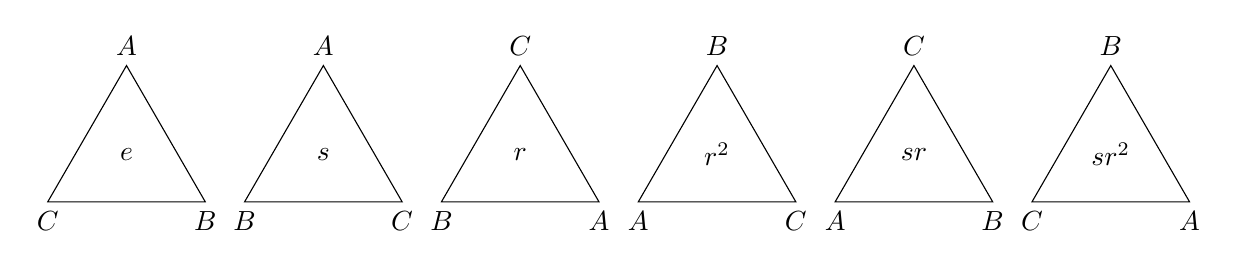
\begin{tikzpicture}
	\draw (0,0) node[below]{\(C\)}
	-- (2,0) node[below]{\(B\)}
	-- (1,1.73) node[above]{\(A\)}
	-- cycle;
	\draw(1, 0.6) node{\(e\)};

	\draw (2.5,0) node[below]{\(B\)}
	-- (4.5,0) node[below]{\(C\)}
	-- (3.5,1.73) node[above]{\(A\)}
	-- cycle;
	\draw(3.5, 0.6) node{\(s\)};

	\draw (5,0) node[below]{\(B\)}
	-- (7,0) node[below]{\(A\)}
	-- (6,1.73) node[above]{\(C\)}
	-- cycle;
	\draw(6, 0.6) node{\(r\)};

	\draw (7.5,0) node[below]{\(A\)}
	-- (9.5,0) node[below]{\(C\)}
	-- (8.5,1.73) node[above]{\(B\)}
	-- cycle;
	\draw(8.5, 0.6) node{\(r^2\)};

	\draw (10,0) node[below]{\(A\)}
	-- (12,0) node[below]{\(B\)}
	-- (11,1.73) node[above]{\(C\)}
	-- cycle;
	\draw(11, 0.6) node{\(sr\)};

	\draw (12.5,0) node[below]{\(C\)}
	-- (14.5,0) node[below]{\(A\)}
	-- (13.5,1.73) node[above]{\(B\)}
	-- cycle;
	\draw(13.5, 0.6) node{\(sr^2\)};
\end{tikzpicture}

As stated before, we assign the letter \(e\) to the identity element.
The operation \(s\) is a reflection; \(r\) is a rotation.
By combining these elements, we get the set of elements of the group.
Note that order matters: \(sr\neq rs\).

\subsection{Definition}
\begin{definition}[Group]
	A group is a set \(G\) together with a way of composing its elements \(\ast\) satisfying (\(\forall g, h, k \in G\)):
	\begin{itemize}
		\item (closure) \(g \ast h \in G\)
		\item (identity) \(\exists e \in G \mathrm{\ s.t.\ } e \ast g = g \ast e = g\)
		\item (inverses) \(\exists g^{-1} \in G \mathrm{\ s.t.\ } g \ast g^{-1} = g^{-1} \ast g = e\)
		\item (associativity) \(g \ast (h \ast k) = (g \ast h) \ast k\)
	\end{itemize}
\end{definition}

Formally, we might say that a set \(G\) with a binary operation \(\ast : G \times G \to G\) is a group if it follows the last three axioms; the first rule is implicit in the function's type.

Here are a few examples of groups.
\begin{enumerate}
	\item \(G = \{ e \}\) --- this is the `trivial group'.
	\item \(G = \{ \text{symmetries of the equilateral triangle} \} \); \(\ast\) is defined by: `\(g \ast h\) means doing \(h\) then \(g\)'.
	\item \(G = (\mathbb Z, +)\).
	      This is easy to prove by verifying the axioms.
	\item \(G = (\mathbb R, +); (\mathbb Q, +); (\mathbb C, +)\)
	\item \(G = (\mathbb R^*, \cdot)\) where \(\mathbb R^* = \mathbb R \setminus \{ 0\}\).
	      Note that \((\mathbb R, \cdot)\) is not a group, because \(\nexists 0^{-1} \in \mathbb R \st 0^{-1} \cdot 0 = 0 \cdot 0^{-1} = 1\).
	\item \(G = (\mathbb R, \ast)\) where \(r \ast s := r + s + 5\).
	\item \(G = (\mathbb Z_n, +)\) where \(\mathbb Z_n = \{ 0, 1, 2, \cdots, n-1 \}\) and addition is done modulo \(n\).
	\item A vector space with the operation of vector addition is a group.
	\item \(GL_2(\mathbb R)\) is the set of invertible \(2\times 2\) matrices, which is a group with respect to matrix multiplication.
\end{enumerate}

Here are a few non-examples.
\begin{enumerate}
	\item \(G = (\mathbb Z_n, +)\) where addition is not performed modulo \(n\).
	      This group is not closed, e.g.
	      \((n-1) + 2 \notin G\).
	\item \(G = (\mathbb Z, \cdot)\) because \(\nexists n\in \mathbb Z \st 2 \cdot n = n \cdot 2 = 1\).
	\item \(G = (\mathbb R, \ast)\) where \(r \ast s = r^2 s\) because there is no identity element.
	\item \(G = (\mathbb N, \ast)\) where \(n \ast m := \abs{n - m}\) because it is non-associative, e.g.
	      \(1 \ast (2 \ast 5) = 2\); \((1 \ast 2) \ast 5 = 4\).
\end{enumerate}

We use the notation \(gh=g\cdot h = g \ast h\) here to represent the group operation (regardless of the specific operation in question).

\subsection{Basic properties}
\begin{proposition}
	Let \(G\) be a group.
	Then,
	\begin{enumerate}
		\item The identity element \(e\) is unique.
		\item \(\forall g \in G\), the inverse \(g^{-1}\) is unique.
		\item \(g \cdot h = g \iff h \cdot g = g\)
		\item \(g \cdot h = e \iff h \cdot g = e\)
		\item \((gh)^{-1} = h^{-1} g^{-1}\)
		\item \((g^{-1})^{-1} = g\)
	\end{enumerate}
\end{proposition}
\begin{proof}
	We prove each case individually.
	\begin{enumerate}
		\item Assume \(\exists e, e'\) which are distinct identity elements.
		      We have \(e e' = e\) and \(e e' = e'\) by the definition of the inverse so \(e = e'\) \contradiction{}
		\item Suppose \(h\) and \(k\) are distinct inverses of \(g\).
		      Then \(gh = e\) and \(gk = e\), so:
		      \begin{align*}
			      gh        & = gk                       \\
			      g^{-1} gh & = g^{-1} gk                \\
			      h         & = k \text{ \contradiction}
		      \end{align*}
		\item \begin{align*}
			      gh      & = g  \\
			      \iff gh & = ge \\
			      \iff h  & = e  \\
			      \iff hg & = eg \\
			      \iff hg & = g
		      \end{align*}
		\item \begin{align*}
			      gh              & = e       \\
			      \iff ghg        & = g       \\
			      \iff g^{-1} ghg & = g^{-1}g \\
			      \iff hg         & = e
		      \end{align*}
		\item \((gh) (h^{-1}g^{-1}) = g h h^{-1} g^{-1} = g g^{-1} = e\)
		\item \(g^{-1} g = e\)
	\end{enumerate}
\end{proof}

\begin{definition}[abelian group]
	A group \(G\) is said to be \textit{abelian} if \(\forall a, b, \in G\), \(a \ast b = b \ast a\).
\end{definition}
A common example of an abelian group is the reals under addition.
A non-example is the group of invertible \(2\times 2\) matrices under matrix multiplication.

\begin{definition}
	The order of a group \(G\), denoted \(\abs{G}\), is the number of elements in the set \(G\).
	A group \(G\) is called a finite group if its order is finite, and it is called an infinite group if its order is infinite.
\end{definition}

\subsection{Subgroups}
\begin{definition}
	Let \((G, \ast)\) be a group.
	A subset \(H \subseteq G\) is a subgroup of \(G\) if \((H, \ast)\) is a group.
	We denote this \(H \leq G\).
\end{definition}
We must verify each group axiom on a subset to check if it is a subgroup --- with the notable exception of the associativity axiom, the property of associativity is inherited by subgroups.
Here are some examples of subgroups.

\begin{enumerate}
	\item \(\{ e \}\) is the trivial subgroup
	\item \(G \leq G\)
	\item \((\mathbb Z, +) \leq (\mathbb Q, +) \leq (\mathbb R, +) \leq (\mathbb C, +)\)
\end{enumerate}
\begin{lemma}
	Let \(G\) be a group.
	\(H \subset G\) is a subgroup of \(G\) if and only if \(H\) is non-empty and \(\forall a, b \in H, ab^{-1} \in H\).
\end{lemma}
\begin{proof}
	We prove each axiom.
	\begin{itemize}
		\item (identity) Setting \(a = b\) gives \(a a^{-1} = e \in H\) as required.
		\item (inverses) Setting \(a = e\), which we know exists from the identity proof above, gives \(b^{-1} \in H\).
		\item (closure) Setting \(b = c^{-1}\), we know that \(c \in H\), and we can always choose a \(b\) such that \(c\) is any value we want; and with the property we can see that \(ac \in H\) as required by the closure axiom.
	\end{itemize}
\end{proof}

\begin{proposition}
	The subgroups of \((\mathbb Z, +)\) are precisely the subsets of the form \(n\mathbb Z \subset Z\) where \(n\mathbb Z := \{nk : k\in \mathbb Z\}\).
\end{proposition}
\begin{proof}
	First, we know that each \(n\mathbb Z\) is a subgroup: given any integer \(n \in \mathbb N\) the axioms hold:
	\begin{itemize}
		\item (closure) given \(nk_1, nk_2 \in n\mathbb Z\), we have \(nk_1 + nk_2 = n(k_1 + k_2) \in n\mathbb Z\)
		\item (identity) \(e = 0 = n \cdot 0 \in n\mathbb Z\)
		\item (inverse) \(-nk = n(-k) \in n\mathbb Z\)
	\end{itemize}
	We also prove the converse statement, namely that the only viable subgroups are of the form \((n\mathbb Z, +)\).
	If \(H = \{ 0 \}\) then clearly \(H = 0\mathbb Z\) which is a trivial subgroup.
	Otherwise, there are some nonzero elements.

	There must be at least one positive element in \(H\), since any negative element can be inverted to make a positive one in \(H\).
	So, let the smallest positive element be \(n\).
	Since \(H\) is a subgroup, it is closed and has inverses.
	This implies that
	\begin{align*}
		n+n+n+\cdots                & \in H; \\
		n^{-1}+n^{-1}+n^{-1}+\cdots & \in H
	\end{align*}
	Therefore \(n\mathbb Z\) is contained within \(H\).
	Now, let us show that there are no extra elements.
	Suppose, for purposes of a contradiction, that \(\exists k \in H \st k \notin n\mathbb Z\).
	Then, since \(k\) is an integer and not a multiple of \(n\), it must lie between two such multiples: \(nm < k < n(m+1)\) where \(m \in \mathbb Z\).
	This means that \(0 < k - nm < n\) which implies that there is a smaller positive element than \(n\) in the set.
	This is a contradiction, so there are no more elements in the set.
\end{proof}

\begin{proposition}
	The following statements are true:
	\begin{itemize}
		\item Let \(H, K\) be subgroups of \(G\).
		      Then \(H \cap K\) is a subgroup of \(G\).
		\item If \(K \leq H\) and \(H \leq G\), then \(K \leq G\).
		\item If \(K \subseteq H\), \(H \leq G\) and \(K \leq G\) then \(K \leq H\).
	\end{itemize}
\end{proposition}
% TODO proofs?
% especially for first part

We can use a lattice diagram to denote subgroups.
Points below other points joined by lines represent subgroups.
Let \(G, H, K\) be groups and \(H \leq G\) and \(K \leq G\).

\begin{center}
	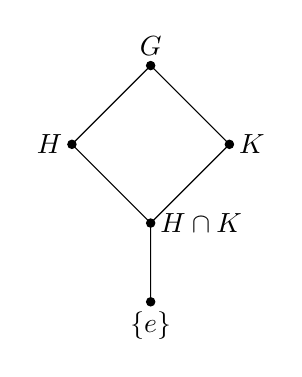
\begin{tikzpicture}
		\draw (0,0) node[below]{\(\{e\}\)}
		-- (0,1) node[right]{\(H \cap K\)}
		-- (1,2) node[right]{\(K\)}
		-- (0,3) node[above]{\(G\)}
		-- (-1,2) node[left]{\(H\)}
		-- (0, 1);
		\filldraw (0,0) circle(1.5pt);
		\filldraw (0,1) circle(1.5pt);
		\filldraw (0,3) circle(1.5pt);
		\filldraw (1,2) circle(1.5pt);
		\filldraw (-1,2) circle(1.5pt);
	\end{tikzpicture}
\end{center}

\subsection{Subgroups generated by a subset}
\begin{definition}
	Let \(X \neq \varnothing\) be a subset of a group \(G\).
	The subgroup \textit{generated by} \(X\) denoted \(\genset{X}\) is the intersection of all subgroups containing \(X\).
	Equivalently, \(\genset{X}\) is the smallest subgroup of \(G\) that contains \(X\) as a subset.
	Note that there will always exist some subgroup \(\genset{X}\) regardless of what \(X\) is chosen; a trivial result would be \(G\) itself.
\end{definition}

We can make a more precise definition of generated groups as follows:
\begin{itemize}
	\item \(\genset{X}\) contains \(e\)
	\item \(\genset{X}\) contains the set \(X\)
	\item \(\genset{X}\) contains all possible products of \(X\) and their inverses
\end{itemize}

\begin{proposition}
	Let \(X \subseteq G, X \neq \varnothing\).
	Then \(\genset{X}\) is the set of elements of \(G\) of the form \(x_1^{\alpha_1} x_2^{\alpha_2} x_3^{\alpha_3} \cdots x_k^{\alpha_k}\) where \(x_i \in X\) (not necessarily distinct), \(\alpha_i = \pm 1\), and \(k \geq 0\).
	By convention, the empty product \(k=0\) is defined to be \(e\).
\end{proposition}
\begin{proof}
	Let \(T\) be the set of such elements of the given form.
	Clearly, \(T \subseteq \genset{X}\).
	Also, \(T\) is a subgroup of \(G\), and \(X \subseteq T\), so \(\genset{X} \subseteq T\).
	Because both \(T \subseteq \genset{X}\) and \(\genset{X} \subseteq T\), we have \(T = \genset{X}\).
\end{proof}
Note that generating sets are not necessarily unique.
For example, the group of integers under addition generated by \(\genset{1}\) is equivalent to \(\genset{2, 3}\), both of which are equivalent to \(\mathbb Z\), for example.
As a discrete example, \(\mathbb Z_5\) can be generated by any element in the set apart from zero, for example: \(\mathbb Z_5 = \genset{1} = \genset{2} = \genset{3} = \genset{4} \neq \genset{0}\).

\section{Homomorphisms}
\subsection{Definition and elementary properties}
\begin{definition}
	Let \((G, \ast_G)\), \((H, \ast_H)\) be groups.
	A function \(\varphi: H \to G\) is a homomorphism if
	\[
		\forall a, b \in H,\quad \varphi(a \ast_H b) = \varphi(a) \ast_G \varphi(b)
	\]
\end{definition}
A homomorphism \(\varphi: H \to G\) may have the following descriptions:
\begin{itemize}
	\item injective, if \(\varphi(a) = \varphi(b) \implies a = b\);
	\item surjective, if \(\forall g \in G, \exists h \in H \st \varphi(h) = g\); and
	\item bijective, if it is both injective and surjective.
\end{itemize}
A more intuitive interpretation of the descriptions is:
\begin{itemize}
	\item A function is injective if the outputs are unique;
	\item A function is surjective if all outputs are used;
	\item A function is bijective if there is a one-to-one relation between every element in the input and output sets.
\end{itemize}
Here are some examples, without proofs.
\begin{enumerate}
	\item Given any two groups \(G\) and \(H\), \(\varphi: H \to G\) defined by \(\varphi(h) = e_G\) is a homomorphism.
	\item The inclusion function \(\iota: H \to G\) where \(H \leq G\) is an injective homomorphism.
	      The inclusion function is defined as the identity function, simply transferring elements from a subgroup into the supergroup.
	\item \(\varphi: \mathbb Z \to \mathbb Z_n\) given that \(\varphi(k) = k \mod n\) is a surjective homomorphism.
	\item \(\varphi: (\mathbb R, +) \to (\mathbb R_{>0}, \cdot)\) where \(R_{>0} = \{r \in \mathbb R : r > 0\}\) and \(\varphi(x) = e^x\) is a bijective homomorphism, otherwise known as an isomorphism.
	\item \(\det : GL_2(\mathbb R) \to (\mathbb R^*, \cdot)\) is a surjective homomorphism.
\end{enumerate}

\begin{proposition}
	Let \(\varphi: H \to G\) be a homomorphism.
	Then, for all \(h \in H\):
	\begin{enumerate}
		\item \(\varphi(e_H) = e_G\)
		\item \(\varphi(h^{-1}) = \varphi(h)^{-1}\)
		\item Given another homomorphism \(\psi: G \to K\), \(\psi \circ \varphi: H \to K\) is a homomorphism.
	\end{enumerate}
\end{proposition}
\begin{proof}
	We prove each result in order.
	\begin{enumerate}
		\item Given the identity element of \(H\) is \(e_H\) and similarly for \(G\),
		      \begin{align*}
			      \varphi(e_H \ast e_H) & = \varphi(e_H) \ast \varphi(e_H) \\
			      \implies \varphi(e_H) & = \varphi(e_H) \ast \varphi(e_H) \\
			      e_G                   & = \varphi(e_H)
		      \end{align*}
		\item Consider \(\varphi(h) \ast \varphi(h^{-1}) = \varphi(h \ast h^{-1}) = \varphi(e_H) = e_G\) which is the defining property of the inverse.
		\item For all \(a, b \in H\):
		      \begin{align*}
			      (\psi \circ \varphi) (a \ast b) & = \psi(\varphi(a \ast b))                           \\
			                                      & = \psi(\varphi(a) + \varphi(b))                     \\
			                                      & = \psi(\varphi(a)) + \psi(\varphi(b))               \\
			                                      & = (\psi \circ \varphi)(a) + (\psi \circ \varphi)(b)
		      \end{align*}
	\end{enumerate}
\end{proof}

\subsection{Isomorphisms}
A bijective homomorphism is called an isomorphism.
If there exists an isomorphism \(\varphi: H \to G\), we say that \(H\) is isomorphic to \(G\), or \(H \cong G\).
\begin{enumerate}
	\item Consider a group \(G\) defined as \(\{ e^{\frac{2 \pi i k}{n}} : k \in \mathbb Z_n \}\) under multiplication.
	      Then, \((G, \cdot) \cong (\mathbb Z_n, +)\) where \(\varphi: \mathbb Z_n \to G\) is defined as \(\varphi(k) = e^{\frac{2\pi i k}{n}}\).
	\item \(\varphi: \mathbb Z \to n\mathbb Z\) for \(n \in \mathbb N\) given by \(\varphi(k) = nk\).
	      Note that all non-trivial subgroups of \(\mathbb Z\) are isomorphic to \(\mathbb Z\).
\end{enumerate}

\begin{proposition}
	Let \(\varphi: H \to G\) be an isomorphism.
	Then \(\varphi^{-1}: G \to H\) is an isomorphism.
\end{proposition}
\begin{proof}
	For all \(a, b \in G\),
	\begin{align*}
		\varphi^{-1}(a \ast b) & = \varphi^{-1}\left[ \varphi(\varphi^{-1}(a)) \ast \varphi(\varphi^{-1}(b)) \right] \\
		                       & = \varphi^{-1}\left[ \varphi(\varphi^{-1}(a) \ast \varphi^{-1}(b)) \right]          \\
		                       & = \varphi^{-1}(a) \ast \varphi^{-1}(b)
	\end{align*}
	So \(\varphi^{-1}\) is a homomorphism.
	But since \(\varphi\) is bijective, so is \(\varphi^{-1}\).
	So \(\varphi^{-1}\) is an isomorphism.
\end{proof}

\subsection{Images and kernels}
\begin{definition}
	Let \(\varphi: H \to G\) be a homomorphism.
	Then the image of \(\varphi\), denoted \(\Im \varphi\), is defined as \(\{ g \in G : g = \varphi(h) \text{ for some } h \in H \}\).
	The kernel of \(\varphi\), denoted \(\ker \varphi\), is defined as \(\{ h \in H : \varphi(h) = e_G \}\).
\end{definition}
Informally, we can say:
\begin{itemize}
	\item The image of \(\varphi\) is the set of outputs of \(\varphi\).
	\item The kernel of \(\varphi\) is the set of inputs that map to the identity element.
\end{itemize}
\begin{proposition}
	\(\Im \varphi \leq G\) and \(\ker \varphi \leq H\).
\end{proposition}
\begin{proof}
	To prove that \(\Im \varphi \leq G\), we check the group axioms (apart from associativity, since this is implicit).
	\begin{itemize}
		\item (closure) If \(a, b \in \Im \varphi\) then there exist some \(x, y \in H\) such that \(\varphi(x) = a\) and \(\varphi(y) = b\).
		      Therefore, \(\varphi(x)\varphi(y)=\varphi(xy)\) which is in the image by definition.
		\item (identity) \(\varphi(e_H) = e_G\)
		\item (inverses) Let \(x \in H\) such that \(\varphi(x) = a\).
		      Then, because \(x^{-1}\in H\), we know that \(\varphi(x^{-1}) = \varphi(x)^{-1} \in \Im H\) as required.
	\end{itemize}
	Now we prove a similar result for the kernel.
	\begin{itemize}
		\item (closure) If \(x, y \in \ker H\) then \(\varphi(xy) = \varphi(x) \varphi(y) = e_G e_G = e_G\), which is the requirement for being in the kernel, so \(xy \in \ker \varphi\).
		\item (identity) \(\varphi(e_H) = e_G\) so the identity element \(e_H\) is in the kernel.
		\item (inverses) \(\varphi(x^{-1}) = \varphi(x)^{-1}\).
		      So if \(x \in \ker \varphi\) then \(\varphi(x^{-1}) = e_G^{-1} = e_G\) so \(\varphi^{-1}\) is also in the kernel.
	\end{itemize}
\end{proof}
Here are a few examples of kernels and images of homomorphisms.
\begin{enumerate}
	\item If \(\varphi: H \to G\) is the trivial homomorphism (mapping every element to the identity) then:
	      \[
		      \Im \varphi = \{ e_G \};\quad \ker \varphi = H
	      \]
	\item If \(H \leq G\) then the inclusion homomorphism \(\iota: H \to G\) has
	      \[
		      \Im \iota = H;\quad \ker \iota = e_H
	      \]
	\item \(\varphi: \mathbb Z \to \mathbb Z_n\) where operations are performed modulo \(n\) has
	      \[
		      \Im \varphi = \mathbb Z_n;\quad \ker \varphi = n\mathbb Z
	      \]
\end{enumerate}

\begin{proposition}
	Let \(\varphi: H \to G\) be a homomorphism.
	Then
	\begin{itemize}
		\item \(\varphi\) is surjective if and only if \(\Im \varphi = G\); and
		\item \(\varphi\) is injective if and only if \(\ker \varphi = \{ e_H \}\).
	\end{itemize}
\end{proposition}
\begin{proof}
	The first case is trivial.
	After all, the definition of surjectivity is that all outputs are mapped onto by something, which means that image is equal to this output set.
	Now, let us prove the injectivity part.
	We start in the forward direction, then we prove the converse.

	Suppose that \(\varphi\) is injective.
	Then \(\varphi(a) = \varphi(b) \implies a = b\).
	We have that \(\varphi(e_H) = e_G\), so \(e_H\) must be the only element sent to \(e_G\).
	Therefore the kernel is simply \(\{ e_H \}\).

	Conversely, suppose that the kernel of \(\varphi\) is simply the identity element.
	Then, let us suppose there are two elements \(a, b\) in \(H\) such that \(\varphi(a) = \varphi(b)\).
	Then, \(\varphi(a b^{-1})=\varphi(a)\varphi(b)^{-1} = \varphi(b)\varphi(b)^{-1} = e_G\).
	Therefore, \(ab^{-1} = e_H\), so \(a = b\).
	So \(\varphi\) is injective.
\end{proof}

\section{Types of groups}
\subsection{Direct products of groups}
\begin{definition}
	The direct product of two groups \(G\) and \(H\) is written \(G \times H\), and defined to be \(\{ (g, h) : g \in G, h \in H \}\), where the group operation is defined by
	\[
		(g_1, h_1) \ast_{G \times H} (g_2, h_2) = (g_1 \ast_G g_2, h_1 \ast_H h_2)
	\]
\end{definition}
We will now prove that this really is a group.
\begin{proof}
	We prove each axiom.
	\begin{itemize}
		\item (closure) For a pair of elements \((g_1, h_1)\) and \((g_2, h_2)\) in \(G \times H\), the product \((g_1 \ast_G g_2, h_1 \ast_H h_2)\) is clearly in \(G \times H\), because the first entry is in \(G\) and the second entry is in \(H\), which is the requirement for being a member of \(G \times H\).
		\item (identity) The element \((e_G, e_H)\) is an identity.
		\item (inverses) Given an element \((g, h) \in G \times H\), the element \((g^{-1}, h^{-1})\) satisfies \((g^{-1}, h^{-1})(g, h) = (e_G, e_H) = e_{G \times H}\).
		\item (associativity) Given three elements \((g_i, h_i)\), \(i \in \{1, 2, 3\}\), we have
		      \begin{align*}
			      ((g_1, h_1) \ast (g_2, h_2)) \ast (g_3, h_3) & = (g_1 \ast g_2, h_1 \ast h_2) \ast (g_3, h_3)       \\
			                                                   & = ((g_1 \ast g_2) \ast g_3, (h_1 \ast h_2) \ast h_3) \\
			                                                   & = (g_1 \ast (g_2 \ast g_3), h_1 \ast (h_2 \ast h_3)) \\
			                                                   & = (g_1, h_1) \ast (g_2 \ast g_3, h_2 \ast h_3)       \\
			                                                   & = (g_1, h_1) \ast ((g_2, h_2) \ast (g_3, h_3))
		      \end{align*}
	\end{itemize}
\end{proof}
\noindent \(G \times H\) contains subgroups \(G \times {e_H}\) and \({e_G} \times H\) which are isomorphic to \(G\) and \(H\) respectively.
We name these subgroups simply \(G\) and \(H\) because they are isomorphic.
\begin{note}
	In \(G \times H\), everything in \(G\) commutes with everything in \(H\).
	\[
		\forall g \in G, \forall h \in H, (g, e_H) \ast (e_G, h) = (e_G, h) \ast (g, e_H) = (g, h)
	\]
\end{note}

\begin{theorem}[Direct Product Theorem]
	Let \(H, K\) be subgroups of \(G\) such that
	\begin{itemize}
		\item \(H \cap K = \{ e \}\) (the groups intersect only in \(e\))
		\item \(\forall h \in H, \forall k \in K, hk = kh\) (\(H\) and \(K\) commute in \(G\))
		\item \(\forall g \in G, \exists h \in H, \exists k \in K \st g = hk\) (\(G = HK\))
	\end{itemize}
	Then \(G \cong H \times K\).
\end{theorem}
\begin{proof}
	Consider \(\varphi: H \times K \to G\) where \(\varphi((h, k)) = hk\).
	We now prove that \(\varphi\) is a homomorphism.
	\begin{align*}
		\varphi((h_1, k_1)(h_2, k_2)) & = \varphi((h_1h_2, k_1k_2))              \\
		                              & = h_1h_2k_1k_2                           \\
		                              & = h_1k_1h_2k_2                           \\
		                              & = \varphi((h_1, k_1))\varphi((h_2, k_2))
	\end{align*}
	Note that by the third property in the theorem we know that \(\varphi\) is surjective.
	We now prove that \(\varphi\) is also injective.

	Suppose that \((h, k) \in \ker \varphi\).
	Then \(\varphi((h, k)) = e_G\) so \(hk = e_G\).
	So \(h = k^{-1}\).
	This means that there is some element that is part of both \(H\) and \(K\), for example \(h\).
	But by the first property in the theorem, this value must be \(e\), so \(\ker \varphi = \{ e_G \}\), so \(\varphi\) is injective.

	\(\varphi\) is an injective, surjective homomorphism, so it is an isomorphism.
	So \(G\) is isomorphic to \(H \times K\).
\end{proof}

\noindent Now, we can consider direct products in two distinct lenses: a combination of smaller groups to form a large one, or a partition of a large group into two that combine to produce the original.

\subsection{Cyclic groups}
\begin{definition}
	Let \(G\) be a group, and let \(X \subseteq G\) be some subset.
	If \(\genset{X} = G\) then \(X\) is a generating set of \(G\).
	We say that \(G\) is cyclic if there exists some element \(a\) in \(G\) such that \(\genset{a} = G\).
	\(a\) is called a generator of \(G\).
\end{definition}
\begin{enumerate}
	\setcounter{enumi}{-1}
	\item The trivial group \(\{ e \}\) is generated by its element.
	\item \((\mathbb Z, +)\) is a cyclic group generated by \(\mathbb Z = \genset{-1} = \genset{1}\).
	\item \((\mathbb Z_n, +)\), where addition is modulo \(n\), is generated by \(\mathbb Z_n = \genset{k}\) where \(k\) and \(n\) are coprime.
\end{enumerate}
\begin{theorem}
	Any cyclic group \(G\) is isomorphic to \(C_n\) (for some \(n \in \mathbb N\)) or \(\mathbb Z\).
\end{theorem}
\begin{proof}
	Let \(G = \genset b\).
	Then suppose that there exists some natural number \(n\) such that \(b^n = e\).
	We take the smallest such \(n\), and define \(\varphi: C_n \to G\) by \(\varphi(a^k) = b^k\) where the elements of \(C_n\) are \(e, a, a^2\) and so on.

	We now show that \(\varphi\) is a homomorphism.
	For any two elements \(a^j, a^k \in C_n\), we have two cases.
	If \(j + k < n\), then \(\varphi(a^j \cdot a^k) = \varphi(a^{j+k}) = b^{j+k} = b^j \cdot b^k = \varphi(a^j) \cdot \varphi(a^k)\) as required.
	Otherwise, \(j + k \geq n\), then \(\varphi(a^j \cdot a^k) = \varphi(a^{j+k-n}) = b^{j+k}(b^n)^{-1} = b^{j+k}\cdot e = b^{j+k} = b^j \cdot b^k = \varphi(a^j) \cdot \varphi(a^k)\) as required.

	Note that \(\varphi\) is bijective:
	\begin{itemize}
		\item \(b^n = e \in G\) implies that all elements of \(G\) can be written \(b^k\) where \(0 \leq k < n\), so \(\varphi\) is surjective; and
		\item Let \(a^k\) be an element in the kernel of \(\varphi\) where \(0 \leq k < n\).
		      Then \(\varphi(a^k) = e \implies b^k = e\).
		      But \(k\) must be zero, because any other value would contradict the fact that we chose \(n\) to be the smallest number with this property.
		      So the kernel is trivial.
	\end{itemize}
	So \(\varphi\) is an isomorphism, and \(G \cong C_n\).

	If alternatively there exists no \(n\) such that \(b^n = e\), then we construct \(\varphi: \mathbb Z \to G\) by \(\varphi(k) = b^k\).
	Then \(\varphi(k + m) = b^{k+m} = b^k \cdot b^m = \varphi(k) \cdot \varphi(m)\), so \(\varphi\) is a homomorphism.
	Clearly \(\varphi\) is surjective because all elements of \(G\) can be constructed with powers of \(b\).
	Now, suppose \(m \in \ker \varphi\) where \(m\) is non-zero.
	Then \(\varphi(m) = b^m = e\) and \(\varphi(-m) = b^{-m} = e\).
	So one of \(m\) and \(-m\) is positive, contradicting the fact that there is no such \(n>0\) where \(b^n = e\).
	So the kernel is trivial, so \(\varphi\) is an isomorphism, so \(G \cong \mathbb Z\).
\end{proof}

\begin{definition}
	The order of an element \(g\in G\) is the smallest \(n \in \mathbb N\) such that \(g^n = e\).
	We say that \(\ord g = n\).
	If there is no such \(n\), then \(\ord g = \infty\).
\end{definition}
Note that given some \(g \in G\), the subgroup \(\genset g\) is a cyclic group isomorphic to \(C_n\) if \(\ord g = n\), and isomorphic to \(\mathbb Z\) if \(\ord g = \infty\).
So \(\ord g = \abs{\genset g}\).
\begin{proposition}
	Cyclic groups are abelian.
\end{proposition}
The proof is trivial.

\subsection{Dihedral groups}
\begin{definition}
	The dihedral group \(D_{2n}\) is the group of symmetries of a regular \(n\)-gon.
	The group operation is composition of transformations.
	For example, \(D_6\) is the group of symmetries of a regular triangle.
\end{definition}
The elements of a general \(D_{2n}\) fall into two categories:
\begin{itemize}
	\item (rotations) We can rotate the shape around its centre through \(\frac{2\pi k}{n}\).
	      There are \(n\) such rotations, including the identity element \(e\).
	\item (reflections) We can reflect the shape across axes through each vertex and the shape's centre.
	      If \(n\) is odd, then there are \(n\) such symmetries.
	      If \(n\) is even, there are \(n/2\) such symmetries, but there are a further \(n/2\) symmetries through the midpoints of edges and the centre of the shape, leaving a total of \(n\).
\end{itemize}
Therefore there are (at least) \(2n\) elements in \(D_{2n}\).
Are these all the elements?
To answer this, let us name vertices \(v_1, v_2 \cdots v_n\), and let us consider some element \(g\) of \(D_{2n}\).
There are two characteristics of a rigid symmetry:
\begin{itemize}
	\item Vertices are mapped to other vertices.
	      So \(v_1 \mapsto v_k\) for some \(1 \leq k \leq n\).
	\item Edges are mapped to other edges.
	      So \(v_2 \mapsto v_{k+1}\) or \(v_{k-1}\) (modulo \(n\)).
	      Note that once we define \(v_1\) and \(v_2\), then the location of \(v_3\) is predetermined.
	      Inductively, the entire polygon is pre-determined.
\end{itemize}
There are \(n\) choices for the location of \(v_1\).
There are two choices for the location of \(v_2\).
So there are only \(2n\) elements in \(D_{2n}\).
So we have all the elements already.
It is also trivial to prove that \(D_{2n}\) is a group, simply by verifying the axioms, noting the function composition is always associative.

Note that we can generate \(D_{2n}\) using just one rotation and one reflection.
Let \(r\) be the rotation by \(\frac{2\pi}{n}\), and let \(s\) be the reflection through \(v_1\) (such that \(v_1 \mapsto v_1\)).
Now,
\begin{itemize}
	\item \(r^k\) gives all possible rotations;
	\item \(r^i s r^{-i}\) gives a reflection through \(v_{i+1}\) and the centre;
	\item \(r^{i+1} s r^{-i}\) gives a reflection through the edge joining \(v_{i}\) and \(v_{i+1}\).
\end{itemize}
These are all three cases, so \(D_{2n} = \genset{r, s}\).

\section{Permutation groups}
\subsection{Definition}
\begin{definition}
	Given a set \(X\), a permutation of the set is a bijective function \(\sigma: X \to X\).
	The set of all permutations of \(X\) is denoted \(\Sym X\).
\end{definition}
\begin{theorem}
	\(\Sym X\) is a group with respect to composition.
\end{theorem}
This is provable by checking the group axioms, noting that all bijective functions are invertible, and that function compositions are always associative.
\begin{definition}
	If \(\abs{X} = n\) then \(S_n\) is the isomorphism class of \(\Sym X\).
\end{definition}
Note that \(\abs{S_n}\) is \(n!
\) because the first element has \(n\) choices for where to be mapped, the second element has \(n-1\) choices, etc.

\subsection{Cycles}
We may use a two-row notation for permutations.
For example, a permutation \(\sigma \in S_3\) such that \(\sigma(1) = 2, \sigma(2) = 3, \sigma(3) = 1\) may be written
\[
	\sigma = \begin{pmatrix}
		1 & 2 & 3 \\
		2 & 3 & 1
	\end{pmatrix}
\]
The columns represent the maps that \(\sigma\) performs: \(1 \mapsto 2; 2 \mapsto 3; 3 \mapsto 1\).
However, this is quite a clunky, long-winded notation.
More often we use a kind of cycle notation, for example
\[
	\sigma = (1\ 2\ 3)
\]
This says that \(\sigma\) represents the cycle \(1 \mapsto 2 \mapsto 3 \mapsto 1\).
Note that, for example, the cycle (1 2 3) is equivalent to the cycle (2 3 1).
We call a cycle like this a 3-cycle because it has 3 elements.
So, for example, the cycle (1 2 3 4 5 6 7) \(\in S_n\) where \(n \geq 7\) is a 7-cycle.
Cycles with two elements are called transpositions, and cycles with one element are called singletons.

Since cycles are permutations, we can compose them like this:
\[
	(1\ 2\ 3\ 4)(3\ 2\ 4) \in S_4
\]
We know that the resulting permutation must be a member of \(S_4\) because of the closure axiom.
We can deduce what the resulting permutation is in two ways:
\begin{itemize}
	\item We can find the value of \((1\ 2\ 3\ 4)(3\ 2\ 4)(x)\) for all \(1 \leq x \leq n\).
	      This allows us to write the permutation in the two-row notation.
	      \[
		      \sigma = \begin{pmatrix}
			      1 & 2 & 3 & 4 \\
			      2 & 1 & 3 & 4
		      \end{pmatrix}
	      \]
	\item Alternatively, let us begin by just finding \(\sigma(1) = 2\).
	      Then, we can find where this result maps to, and so on, until we have a completed cycle.
	      We are guaranteed to form a cycle, as we will prove later.
	      Repeat this cycle generation for all unused numbers, and then you will get a product of cycles, in this case \(\sigma = (1\ 2)(3)(4)\).
\end{itemize}
Note that the inverse of a permutation can be created by swapping the rows.
A cycle can be inverted by simply reversing the order of its elements.
One more interesting fact is that \(D_{2n} \leq S_n\).
\(D_{2n}\) is a permutation of \(n\) vertices with some added constraints (e.g.
edges must map to edges), so it makes sense that it would be a subgroup.
In particular, \(D_6 = S_3\).

\subsection{Disjoint cycles}
Cycles are considered disjoint if no number appears in both.
\begin{lemma}
	Disjoint cycles commute.
\end{lemma}
\begin{proof}
	Let \(\sigma, \tau\) be disjoint cycles of \(S_n\).
	We want to prove that \(\sigma\tau(x) = \tau\sigma(x)\) for all \(1 \leq x \leq n\).
	There are three cases:
	\begin{itemize}
		\item If \(x \notin \sigma\) and \(x \notin \tau\) then immediately \(\sigma\tau(x) = x = \tau\sigma(x)\).
		\item If \(x \in \sigma\) but \(x \notin \tau\) then because \(\sigma\) is a cycle, \(\sigma(x) \in \sigma\); and because the cycles are disjoint, \(\sigma(x) \notin \tau\).
		      So \(\sigma\tau(x) = \sigma(x) = \tau\sigma(x)\).
		\item If \(x \in \tau\) but \(x \notin \sigma\), use the proof above but swap the letters.
	\end{itemize}
\end{proof}

\subsection{Disjoint cycle decomposition}
\begin{theorem}
	Any \(\sigma \in S_n\) can be written as a product of disjoint cycles.
	This is unique up to reordering cycles (and, of course, moving the elements around within a cycle without altering it).
\end{theorem}
\begin{proof}
	Let \(\sigma \in S_n\).
	Now consider the infinite list of terms \(1, \sigma(1), \sigma^2(1), \sigma^3(1) \cdots\).
	\(\sigma\) is a bijection from a set to itself so this list will continue infinitely, but there are only \(n\) possible items in this set.
	Therefore, by the pigeonhole principle, there must be two distinct items in that list that are the same.
	Let us label their indices \(a\) and \(b\), such that \(\sigma^a(1) = \sigma^b(1)\), and that \(a > b\) without loss of generality.
	Then we can multiply on the right by \(\sigma^{-b}(1)\) to get \(\sigma^{a-b}(1) = 1\).

	Now that we have proven that the number 1 exists multiple times in the list, let us take \(k\) to be the smallest positive integer such that \(\sigma^k(1) = 1\).
	Then for \(0 \leq l < m < k\), if \(\sigma^m(1) = \sigma^l(1)\) then \(\sigma^{m-l}(1) = 1\) which contradicts the minimality of \(k\).
	So the first \(k\) numbers on the list are distinct, so \((1\ \sigma(1)\ \sigma^2(1)\ \cdots\ \sigma^{k-1}(1))\) is a cycle.

	Repeat this whole process, replacing 1 with different unused values in the set.
	This will always continue to work because no number that has already appeared can reappear (because \(\sigma\) is a bijection).

	Continue until we have exhausted the entire set \(\{ 1, \cdots, n\}\).
	Then we can multiply together all of the (disjoint) cycles we have generated.
	Note that each element from \(\{ 1, \cdots, n\}\) must appear exactly once in this product (if it is mapped to itself, it is present as a singleton).
	It is clear then that this product is equal to \(\sigma\), because for any input \(k\), no cycles except for the one containing said input (and also, of course, containing the output \(\sigma(k)\)) will do anything to it.

	We can prove the uniqueness of the decomposition by supposing that there might exist two decompositions.
	Taking any element \(x\) in the set \(\{ 1, \cdots, n\}\), we know that \(\sigma\) uniquely defines the cycle that \(x\) belongs to.
	So that means that in both decompositions, the cycle containing \(x\) is the same.
	By repeating this for all \(x\) in the set, we can be sure that all cycles are the same, and thus the decompositions in their entirety are the same.
	Therefore the decomposition is unique.
\end{proof}

\subsection{Order of permutations}
The set of cycle lengths of the disjoint cycle decomposition of \(\sigma\) is called the cycle type of \(\sigma\).
For example, \(\sigma = (1\ 2\ 3)(5\ 6)\) has cycle type \(3, 2\) (or equivalently \(2, 3\)).

\begin{theorem}
	The order of \(\sigma \in S_n\) is the least common multiple of the cycle lengths in its cycle type.
\end{theorem}
\begin{proof}
	The order of a \(k\)-cycle is \(k\).
	Let us decompose \(\sigma\) into a product of disjoint cycles such that \(\sigma = \tau_1 \tau_2 \cdots \tau_r\).
	Then \(\sigma^m = \tau_1^m \tau_2^m \cdots \tau_r^m\) since disjoint cycles commute.

	Let each \(\tau_i\) be a \(k_i\)-cycle.
	Then if \(\sigma^m = e\), \(\tau_1^m \tau_2^m \cdots \tau_r^m = e\), and so \(\tau_1^m = \tau_2^{-m} \tau_3^{-m} \cdots \tau_r^{-m}\).
	Note that the right hand side and left hand side permute different elements, so they must both be the identity element \(e\).
	Repeating this style of argument with every \(\tau\) shows that \(\tau_i^m = e\) so \(k_i | m\).

	So clearly the lowest common multiple of all of the \(k_i\) divides the order of the permutation, \(o(\sigma)\).
	Now, we check that it is actually equal to \(o(\sigma)\).
	Let \(L\) be this lowest common multiple.
	Then \(\sigma^L = \tau_1^L \tau_2^L \cdots \tau_r^L = (\tau_1^{k_1})^{L/k_1} (\tau_2^{k_2})^{L/k_2} \cdots (\tau_r^{k_r})^{L/k_r}\).
	All of these exponents are integers because \(L\) is a multiple of each \(k_i\).
	So we have \(e \cdot e \cdots e = e\).
	So the order of \(\sigma\) is \(L\).
\end{proof}

\subsection{Products of transpositions}
\begin{proposition}
	Let \(\sigma \in S_n\).
	Then \(\sigma\) is a product of transpositions.
\end{proposition}
\begin{proof}
	It is enough to prove this for just a cycle, then we can use the disjoint cycle decomposition to create a transposition product for the whole \(\sigma\).
	\((a_1\ a_2\cdots a_n) = (a_1\ a_2)(a_2\ a_3)\cdots(a_{n-1}\ a_n)\), so the result is immediate.
\end{proof}
\noindent Note that this decomposition is not unique in general.

\subsection{Permutation parity}
A permutation may be considered even if its transposition decomposition has an even number of terms, or odd otherwise.
Note that an even-length cycle has odd parity, and an odd-length cycle has even parity.
\begin{proposition}
	The parity of a permutation is well-defined, regardless of exactly how you write a permutation.
\end{proposition}
\begin{proof}
	Let us denote the amount of cycles in the disjoint cycle decomposition of \(\sigma\) with \(\#(\sigma)\).
	Let \(\tau = (c\ d)\).
	Then the effects of multiplying \(\sigma\) by \(\tau\) (on the right) have two cases, since it only affects \(c\) and \(d\).
	\begin{itemize}
		\item If \(c\) and \(d\) are in the same cycle in \(\sigma\), we get the following conversion:
		      \[
			      (c\ a_2 \cdots a_{k-1}\ d\ a_{k+1} \cdots a_l) \mapsto (c\ a_{k+1} \cdots a_l) (d\ a_2 \cdots a_{k-1})
		      \]
		      So \(\#(\sigma\tau) = \#(\sigma) + 1\).
		\item Otherwise, \(c\) and \(d\) are in different cycles (possibly singletons) in \(\sigma\), so we get the following conversion:
		      \[
			      (c\ a_2 \cdots a_k) (d\ b_2 \cdots a_l) \mapsto (c\ b_2 \cdots b_l\ d\ a_2 \cdots a_k)
		      \]
		      So \(\#(\sigma\tau) = \#(\sigma) - 1\).
	\end{itemize}
	In either case, parity is flipped.
	Now, suppose that \(\sigma\) is written as two products of transpositions, where one has \(m\) transpositions, and one has \(n\) transpositions.
	Therefore we have \(\#(\sigma) \equiv \#(e) + m \text{ mod } 2\), and \(\#(\sigma) \equiv \#(e) + n \text{ mod } 2\).
	But \(\#(\sigma)\) is uniquely determined by \(\sigma\), so both equations match, so \(m \equiv n \text{ mod } 2\), so the parity is well-defined.
\end{proof}

\begin{definition}
	Writing \(\sigma\) as a product of transpositions, the sign of \(\sigma\) is defined as 1 if the permutation is even, and \(-1\) if it is odd.
\end{definition}
Note that the function \(\mathrm{sign}(\sigma)\) is a homomorphism from \(S_n\) to \((\{-1, 1\}, \cdot)\).

\begin{definition}
	The alternating group \(A_n\) is defined as the kernel of the sign homomorphism on \(S_n\).
	In other words, it is the set of even permutations of \(S_n\).
\end{definition}

\section{M\"obius transformations}
\subsection{The M\"obius group}
M\"obius groups are an analogous concept to permutation groups, but on the infinite set of the complex numbers.
A M\"obius transformation \(f\) is defined as follows:
\[
	f: \Chat \to \Chat;\quad f(z) = \frac{az + b}{cz + d};\quad a, b, c, d \in \mathbb C;\quad ad-bc \neq 0
\]
The reason for the restriction that \(ad-bc\neq 0\) is that \(ad=bc\) implies that \(f\) is a constant value for all \(z\).
Note that \(\Chat\) is known as the `extended complex plane', defined as the complex plane together with a point at infinity, denoted \(\infty\).
There are some special points related to M\"obius transformations:
\begin{itemize}
	\item \(f(\frac{-d}{c})\) is defined to be \(\infty\).
	      This is because the denominator of the fraction would be zero.
	\item \(f(\infty)\) is defined to be \(\frac{a}{c}\) if \(c \neq 0\).
	      This is because as the length of \(z\) increases to infinity, the constant terms \(b\) and \(d\) vanish.
	      However, if \(c = 0\), then the numerator explodes to infinity as the denominator remains constant, so \(f(\infty) = \infty\) in this case.
\end{itemize}

\begin{lemma}
	M\"obius transformations are bijections from \(\Chat \to \Chat\).
\end{lemma}
\begin{proof}
	We can prove this by evaluating \(f(f^{-1}(z))\) and \(f^{-1}(f(z))\) at all \(z\), taking into account all the special points.
	The entire proof is not written here, but it suffices to substitute every special point and a generic \(z\) into both of these expressions, and show that they equal \(z\) in all cases.
\end{proof}

\begin{theorem}
	The set \(\mathcal M\) of M\"obius maps forms a group under composition of functions.
\end{theorem}
\begin{proof}
	We must check each of the group axioms, and we begin with closure.
	Let \(f_1(z) = \frac{a_1 z + b_1}{c_1 z + d_1}; f_2(z) = \frac{a_2 z + b_2}{c_2 z + d_2}\).
	To compose these functions, we first ignore the special points and then check them individually later.
	\begin{align*}
		(f_2 \circ f_1)(z) & = f_2(f_1(z))                                                                                                               \\
		                   & = \frac{a_2 \left( \frac{a_1 z + b_1}{c_1 z + d_1} \right) + b_2}{c_2 \left( \frac{a_1 z + b_1}{c_1 z + d_1} \right) + d_2} \\
		                   & = \frac{(a_1 a_2 + b_2 c_1)z + (a_2 b_1 + b_2 d_1)}{(c_2 a_1 + d_2 c_1)z + (c_2 b_1 + d_1 d_2)}                             \\
		                   & =: \frac{az + b}{cz + d}
	\end{align*}
	Note that \(ad-bc = (a_1 a_2 + b_2 c_1)(c_2 b_1 + d_1 d_2) - (a_2 b_1 + b_2 d_1)(c_2 a_1 + d_2 c_1) = (a_1 d_1 - b_1 c_1)(a_2 d_2 - b_2 c_2)\) which is the product of two nonzero numbers, which is therefore nonzero.
	Now we will check all the special points.
	\begin{align*}
		(f_2 \circ f_1)(\infty)                                         & = f_2\left(\frac{a_1}{c_1}\right)                                                           \\
		                                                                & = \frac{a_2 \left( \frac{a_1}{c_1} \right) + b_2}{c_2 \left( \frac{a_1}{c_1} \right) + d_2} \\
		                                                                & = \frac{a_1 a_2 + b_2 c_1}{c_2 a_1 + d_2 c_1}                                               \\
		                                                                & = \frac{a}{c}                                                                               \\
		(f_2 \circ f_1)(\infty)                                         & = f_2(\infty) = \frac{a_2}{c_2}                                                             \\
		(f_2 \circ f_1)\left(f^{-1}\left(\frac{-d_2}{c_2}\right)\right) & = f_2\left( \frac{-d_2}{c_2} \right)                                                        \\
		                                                                & = \infty
	\end{align*}
	Note that each of these results matches up with our intuitive understanding of infinity in the limit, for instance \((f_2 \circ f_1)(\infty) = \frac{a}{c}\), where na\"\i{}vely we might assume \((f_2 \circ f_1)(\infty) = \frac{a \cdot \infty + b}{c \cdot \infty + d} = \frac{a}{c}\).

	Now we may prove the other group axioms hold for \(\mathcal M\).
	Clearly there is an identity element \(f(z) = \frac{1z + 0}{0z + 1}\).
	We know that there are always inverses because \(f\) is a bijection.
	Finally, we know that all M\"obius maps obey the associative law because function composition is always associative.
	So \(\mathcal M\) is a group.
\end{proof}

\subsection{Properties of the M\"obius group}
When we are working with M\"obius groups, we use the following conventions:
\[
	\frac{1}{\infty} = 0;\quad \frac{1}{0} = \infty;\quad \frac{a\cdot\infty}{c\cdot\infty} = \frac{a}{c}
\]

Firstly, \(\mathcal M\) is not abelian.
For example, let \(f_1(z) = z + 1; f_2(z) = 2z\).
Then \((f_2 \circ f_1)(z) = 2z + 2\) and \((f_1 \circ f_2)(z) = 2z + 1\).

\begin{proposition}
	Every M\"obius transformation can be written as a composition of maps of the following forms:
	\begin{enumerate}[(i)]
		\item \(f(z) = az\) where \(a\neq 0\).
		      This is a dilation or rotation.
		\item \(f(z) = z + b\).
		      This is a translation by \(b\).
		\item \(f(z) = \frac{1}{z}\).
		      This is an inversion.
	\end{enumerate}
\end{proposition}
\begin{proof}
	Let \(f(z) = \frac{az + b}{cz + d}\).
	Then if \(c \neq 0\), \(f(z)\) is given by
	\[
		z \xrightarrow{\text{(ii)}} z + \frac{d}{c} \xrightarrow{\text{(iii)}} \frac{1}{z + \frac{d}{c}} \xrightarrow{\text{(i)}} \frac{(-ad+bc)c^{-2}}{z + \frac{d}{c}} \xrightarrow{\text{(ii)}} \frac{a}{c} + \frac{(-ad+bc)c^{-2}}{z + \frac{d}{c}} = \frac{az + b}{cz + d}
	\]
	If \(c = 0\), \(f(z)\) is given by
	\[
		z \xrightarrow{\text{(i)}} \frac{a}{d}z \xrightarrow{\text{(ii)}} \frac{a}{d}z + \frac{b}{d} = \frac{az + b}{d}
	\]
\end{proof}
Note therefore that the set \(\mathcal S\) of all dilations, rotations, translations and inversions generates \(\mathcal M\), or in symbolic form, \(\genset {\mathcal S} = \mathcal M\).

\section{Cosets and Lagrange's theorem}
\subsection{Cosets}
Let \(H\) be a subgroup of some group \(G\), and let \(g \in G\).
Then a set of the form \(gH := \{ gh : h \in H \}\) is called a left coset of \(H\) in \(G\).
Also, a set of the form \(Hg := \{ hg : h \in H \}\) is called a right coset of \(H\) in \(G\).
Mostly we use left cosets, but right cosets can be seen in more specific scenarios.
Note that the order of group \(H\) is the same as the order of the cosets \(gH\) and \(Hg\); we can think of \(gH\) and \(Hg\) as translated copies of \(H\).
Note further that \(gH\) and \(Hg\) are not necessarily groups; in fact in general they are not groups.
We now consider some example cosets.
\begin{enumerate}
	\item Let \(H = \{ e \} \leq G\).
	      Then \(gH = \{ g \}\).
	\item Let \(H = 2\mathbb Z\) and let \(G = \mathbb Z\).
	      Then (where the cosets are written additively):
	      \begin{itemize}
		      \item \(0 + 2\mathbb Z = 2\mathbb Z\) which is the set of even integers.
		      \item \(1 + 2\mathbb Z = \{ 1 + k: k \in 2\mathbb Z \}\) which is the set of odd integers.
		      \item \(2 + 2\mathbb Z = 2\mathbb Z\).
		            There are only two distinct cosets of \(H\) in \(G\) here; every odd integer will create the set of odd integers, and every even integer will create the set of even integers.
	      \end{itemize}
	\item Let \(H = \{ e, (1\ 2) \}\), and let \(G = S_3\).
	      Then, each (left) coset of \(H\) in \(G\) is given by
	      \begin{itemize}
		      \item \(eH = \{ e, (1\ 2) \} = H\)
		      \item \((1\ 2)H = \{ (1\ 2), e \} = H\)
		      \item \((1\ 3)H = \{ (1\ 3), (1\ 2\ 3) \}\)
		      \item \((1\ 2\ 3)H = \{ (1\ 2\ 3), (1\ 3) \}\)
		      \item \((2\ 3)H = \{ (2\ 3), (1\ 3\ 2) \}\)
		      \item \((1\ 3\ 2)H = \{ (1\ 3\ 2), (2\ 3) \}\)
	      \end{itemize}
	      Note that:
	      \begin{itemize}
		      \item \(eH = H\)
		      \item \(\forall h \in H, hH = H\) as \(H\) is a group and therefore closed under multiplication with \(h\)
		      \item \(\abs{gH} = \abs{H}\)
		      \item \(\bigcup_{g\in G} gH = G\), and in this example in particular, each pair of cosets is equal and disjoint to any other pair
	      \end{itemize}
\end{enumerate}

\subsection{Lagrange's theorem}
\begin{definition}
	We define the index of a subgroup \(H \leq G\) in \(G\), written \(\abs{G : H}\), to be the number of distinct cosets of \(H\) in \(G\).
\end{definition}
\begin{theorem}[Lagrange's Theorem]
	Let \(H \leq G\) be a subgroup of a finite group \(G\).
	Then:
	\begin{enumerate}
		\item \(\abs{H} = \abs{gH}\) for any \(g \in G\);
		\item for any \(g_1, g_2 \in G\), either \(g_1 H = g_2 H\) or \(g_1 H \cap g_2 H = \varnothing\); and
		\item \(G = \bigcup_{g \in G} gH\)
	\end{enumerate}
	And in particular, \(\abs{G} = \abs{G : H} \cdot \abs{H}\).
\end{theorem}
\begin{proof}
	We prove each statement independently.
	\begin{enumerate}
		\item The function \(H \to gH\), defined by \(h \mapsto gh\), defines a bijection between \(H\) and \(gH\), so \(\abs{H} = \abs{gH}\).
		\item Suppose \(g_1 H \cap g_2 H \neq \varnothing\).
		      Then \(\exists g \in g_1 H \cap g_2 H\).
		      So \(g = g_1 h_1 = g_2 h_2\) for some \(h_1, h_2 \in H\).
		      So \(g_1 = g_2 h_2 h_1^{-1}\).
		      So for any \(h \in H\), we have
		      \[
			      g_1 h = g_2 \underbrace{h_2 h_1^{-1} h}_{\mathclap{\in H}}
		      \]
		      So certainly \(g_1 H \subseteq g_2 H\).
		      Employing a symmetric argument for the other way round, we have \(g_1 H = g_2 H\).
		\item Given some \(g \in G\) then \(g \in gH\), since \(e \in H\).
		      So \(G \subseteq \bigcup_{g \in G} gH\).
		      But also, \(gH \subseteq G\), so \(\bigcup_{g \in G} gH \subseteq G\).
		      So \(G = \bigcup_{g \in G} gH\).
	\end{enumerate}
	So now that we know that \(G\) is composed of a union of disjoint cosets, all of which are the same size, we know that \(\abs{G}\) is just the number of these cosets multiplied by the size of such a coset, or in other words
	\[
		\abs{G} = \abs{G : H} \cdot \abs{H}
	\]
\end{proof}
Note that we could equivalently have used right cosets in place of left cosets.
Remember that in general, \(gH \neq Hg\), and the set of left cosets is not equal to the set of right cosets.
\begin{proposition}
	\(g_1 H = g_2 H \iff g_1^{-1} g_2 \in H\).
\end{proposition}
\begin{proof}
	We first consider the forwards case.
	Clearly \(g_1\) is an element of \(g_1 H\), as \(H\) contains \(e\).
	Also, \(g_2\) is an element of \(g_2\).
	So \(g_1^{-1} g_2 \in H\).
	Now for the backwards case.
	Clearly, \(g_2 H\) contains the element \(g_2\), as \(e\) maps to it.
	Also, since \(H\) contains \(g_1^{-1} g_2\), \(g_1 H\) contains the element \(g_1 \ast (g_1^{-1} g_2) = g_2\).
	As cosets are either disjoint or equal, and they clearly share the element \(g_2\), then they are equal.
\end{proof}
Note further that \(g' \in gH\) implies \(g'H = gH\).
We may therefore take a single element from each of these distinct cosets, and we will call them \(g_1, g_2, \cdots, g_{\abs{G:H}}\).
Then
\[
	G = \bigsqcup_{i=1}^{\abs{G:H}} g_i H
\]
where the \(\bigsqcup\) symbol denotes a disjoint union of sets.
These \(g_i\) are called coset representatives of \(H\) in \(G\).

\begin{corollary}
	Let \(G\) be a finite group and \(g \in G\).
	Then \((\ord g) \mid \abs{G}\).
\end{corollary}
\begin{proof}
	Recall that \(\ord g\) is defined as the smallest \(n\) such that \(g^n = e\).
	We define the subgroup \(H \leq G\) as \(H = \genset g\).
	Then \(\ord g = \abs{H}\).
	By Lagrange's Theorem, we know that \(\abs{H} \mid \abs{G}\).
\end{proof}

\begin{corollary}
	Let \(G\) be a finite group, and let \(g \in G\).
	Then \(g^{\abs{G}} = e\).
\end{corollary}
\begin{proof}
	This follows directly from the previous corollary.
	\(g^{\abs{G}} = g^{n \cdot \ord g}\) for some natural number \(n\), so this simply reduces to \(e\).
\end{proof}

\begin{corollary}
	Groups of prime order are cyclic, and are generated by any non-identity element.
\end{corollary}
\begin{proof}
	Let \(\abs{G} = p\), where \(p\) is a prime.
	We will take some \(g \in G\), and generate a group from it.
	By Lagrange's Theorem, \(\abs{\genset{g}} \mid \abs{G}\), so \(\abs{\genset g}\) is either 1 or \(p\).
	Now, note that \(e\) and \(g\) are both elements of \(\genset{g}\), so if \(g \neq e\) then clearly \(\abs{\genset{g}} > 1\), so \(\abs{\genset{g}} = p\).
\end{proof}
We can take Lagrange's theorem into the world of number theory, and specifically modular arithmetic, where we are dealing with finite groups.
Clearly, \(\mathbb Z_n\) is a group under addition modulo \(n\), but what happens with multiplication modulo \(n\)?
Clearly this is not a group --- for a start, 0 has no inverse.
By removing all elements of the group that have no inverse, we obtain \(\mathbb Z_n^*\).

Note that for any \(x \in \mathbb Z_n\), \(x\) has a multiplicative inverse if and only if \(\HCF(x, n) = 1\), i.e.\ if \(x\) and \(n\) are coprime.
This follows directly from the fact that we can write 1 as a linear combination of \(x\) and \(n\), i.e.\ \(xy + mn = 1\), thus defining \(y\) as the multiplicative inverse of \(x\) modulo \(n\).
From this, it is simple to check that \(\mathbb Z_n^*\) forms a group under multiplication.

We may also create an equivalent group-theoretic definition of Euler's totient function \(\varphi\) as follows: \(\varphi(n) := \abs{\mathbb Z_n^*}\).
We can now use Lagrange's theorem to prove the Fermat--Euler theorem (that is, \(\HCF(N, n) = 1 \implies N^{\varphi(n)} \equiv 1 \mod n\)) as follows.
\begin{proof}
	If \(N\) and \(n\) are coprime, then there is an element, here denoted \(a\), in \(\mathbb Z_n\) corresponding to \(N\).
	So \(a^{\varphi(n)} = a^{\abs{\mathbb Z_n^*}} = 1\) in \(\mathbb Z_n\).
	Since \(N = a + kn\), we may expand \(N^{\varphi(n)} = a^{\varphi(n)} + n(\cdots) \equiv a^{\varphi(n)} \equiv 1 \mod n\).
\end{proof}

\subsection{Groups of small order}
We can completely classify groups of small order; we already know enough to classify all groups up to order 5 using Lagrange's Theorem.
\begin{proposition}
	If \(\abs{G} = 4\), then \(G \cong C_4\) or \(G \cong C_2 \times C_2\).
\end{proposition}
\begin{proof}
	By Lagrange's Theorem, the possible orders of elements of \(G\) with \(\abs{G} = 4\) are 1 (only the identity), 2 and 4.
	\begin{itemize}
		\item If there is an element \(g\) of order 4, then \(G = \genset{G}\) because \(e \neq g \neq g^2 \neq g^3\), so it is cyclic of order 4.
		\item If there is no such element, then all non-identity elements must have order 2.
		      \(G\) is abelian (by question 7 on example sheet 1).
		      Take two distinct elements \(b, c\) of order 2.
		      Then:
		      \begin{itemize}
			      \item \(\genset b \cap \genset c = \{ e, b \} \cap \{ e, c \} = \{ e \}\)
			      \item \(bc = cb\) as the group is abelian.
			      \item The element \(bc\) is not equal to \(b\) or \(c\) (\(bc = b \implies c = e\) which is an element of order 1).
			            It is also not equal to \(e\) because then \(b = c^{-1}\) which implies \(b = c\).
			            So the remaining element of \(G\) is simply \(bc\).
			            So any element in \(G\) may be written as the product of an element in \(\genset b\) multiplied by an element in \(\genset c\).
		      \end{itemize}
		      These are the three conditions of the direct product theorem, so \(G = \genset b \times \genset c \cong C_2 \times C_2\).
	\end{itemize}
\end{proof}
Now here is a list the first five smallest groups (we need more tools in order to classify larger groups):
\begin{enumerate}
	\item \(G = \{ e \}\)
	\item \(G \cong C_2\) because a group of prime order is cyclic.
	\item \(G \cong C_3\) for the same reason.
	\item \(G \cong C_4\) or \(G \cong C_2 \times C_2\) by the proof above.
	\item \(G \cong C_5\) because 5 is prime.
\end{enumerate}

\section{Normal subgroups and quotients}
\subsection{Normal subgroups}
How and when does it make sense to divide one group by another?
\begin{definition}
	An subgroup \(N\) of a group \(G\) is \textit{normal} if \(\forall g \in G, gN = Ng\).
	We write \(N \trianglelefteq G\).
\end{definition}
\noindent The following equivalent definitions hold:
\begin{itemize}
	\item \(\forall g \in G, gN = Ng\)
	\item \(\forall g \in G, \forall n \in N, g^{-1}ng \in N\)
	\item \(\forall g \in G, g^{-1}Ng = N\)
\end{itemize}
\begin{proof}
	The first case is the definition.
	For the second case, clearly (from the first definition) \(ng \in gN\).
	So multiplying on the left by \(g^{-1}\), we have \(g^{-1}ng \in N\) as required.
	For the third case, we can simply multiply the first definition on the left by \(g^{-1}\).
	Note that these multiplications are distributed over each element in the coset: \(a(bC) = \{ abc : c \in C \}\).
\end{proof}

\begin{enumerate}
	\item \(\{ e \}\) and \(G\) are normal subgroups of \(G\).
	\item \(n\mathbb Z \trianglelefteq \mathbb Z\).
	      \(\forall a \in \mathbb Z\), we have \(a + n\mathbb Z = \{ a + nk : k \in \mathbb Z \} = \{ nk + a : k \in \mathbb Z \} = n\mathbb Z + a\).
	\item \(A_3 \trianglelefteq S_3\).
	      \begin{itemize}
		      \item \(eA_3 = A_3 = A_3 e\)
		      \item \((1\ 2\ 3)A_3 = A_3 = A_3(1\ 2\ 3)\)
		      \item \((1\ 3\ 2)A_3 = A_3 = A_3(1\ 3\ 2)\)
		      \item \((1\ 2)A_3 = \{ (1\ 2), (2\ 3), (1\ 3) \} = A_3(1\ 2)\)
	      \end{itemize}
	      and so on.
\end{enumerate}

\begin{proposition}
	\begin{enumerate}
		\item Any subgroup of an abelian group is normal.
		\item Any subgroup of index 2 is normal.
	\end{enumerate}
\end{proposition}
\begin{proof}
	\begin{enumerate}
		\item If \(G\) is abelian, then \(\forall g \in G, \forall n \in N, g^{-1}ng = n \in N\) which is stronger than required.
		\item If \(H \leq G\) with \(\abs{G : H} = 2\), then there are only 2 cosets.
		      \(H = eH = He\) is one of the two cosets.
		      Since cosets are disjoint, the other coset must be \(G \setminus H\).
		      This is true for both left and right cosets.
		      So the other left and right cosets must be equal, so \(H\) is normal.
	\end{enumerate}
\end{proof}

\begin{proposition}
	If \(\varphi: G \to H\) is a homomorphism, then \(\ker \varphi \trianglelefteq G\).
\end{proposition}
\begin{proof}
	We already know \(\ker \varphi\) is a subgroup of \(G\).
	Now we must check it is normal.
	Given some \(k \in \ker \varphi, g \in G\), we want to show that \(g^{-1} k g \in \ker \varphi\).
	We have \(\varphi(g^{-1} k g) = \varphi(g^{-1}) \varphi(k) \varphi(g) = \varphi(g^{-1}) e \varphi(g) = \varphi(g^{-1}g) = \varphi(e) = e\) so \(g^{-1} k g \in \ker \varphi\) as required.
\end{proof}
In fact, we will show later that normal subgroups are exactly kernels of homomorphisms and nothing else.

Here is now a less formal explanation of this theorem and its consequences.
Consider some subgroup \(K \leq G\).
There may be some property \(P\) that is true for every element of \(K\) and false for every other element of \(G\).
Then certainly, for example, given \(k_1, k_2 \in K\), we know that \(k_1k_2\) has the same property as it is within \(K\).
As another example, let \(k \in K\) and let \(g \in G \setminus K\).
Then \(kg\) does not have this property, as \(kg \notin K\).

We can encapsulate this behaviour by making a homomorphism from the whole group \(G\) to some other group --- it \textit{doesn't matter where we end up}, just as long as anything with this particular property maps to the new group's identity element.
Let \(\varphi: G \to H\), where \(H\) is some group that we don't really care about (apart from the identity).
This means that any element of \(K\), i.e.\ any element with property \(P\), is mapped to \(e_H\).
By the laws of homomorphisms, any product of \(k \in K\) with \(g \in G \setminus K\) does not give the identity element, so it does not have this property!
This is exactly the behaviour we wanted.

If we can find such a homomorphism, then \(K\) is the kernel of this homomorphism.
Again, the image of this homomorphism is essentially irrelevant; all we care about is which elements map to the identity.
Now, note that by the laws of homomorphisms, given some element \(g \in G\) and \(k \in K\), \(\varphi(g^{-1}kg) = \varphi(g^{-1})\varphi(k)\varphi(g)\).
But since \(k\) has this desired property, the \(\varphi(k)\) term vanishes.
So we're left with the identity element.
This gives us the result that \(g^{-1}kg\) must be an element of \(K\), so it must have property \(P\).
This is a definition for a normal subgroup, so \(K\) must be normal in order for us to be able to find such a homomorphism \(\varphi\).

As another small aside, a normal subgroup in this context essentially means this: given some element \(k\) with property \(P\), the property is preserved when surrounding \(k\) with inverses.
This is just a `translation' of a definition of a normal subgroup: \(g^{-1}kg \in K\).

\begin{enumerate}
	\item \(SL_n(\mathbb R) \trianglelefteq GL_n(\mathbb R)\), where \(GL_n(\mathbb R)\) is the group of invertible matrices of dimension \(n\), and where \(SL_n(\mathbb R)\) is the group of matrices of determinant 1.
	      This is because \(\det: GL_n(\mathbb R) \to \mathbb R^*\), and \(SL_n(\mathbb R) = \ker (\det)\).
	\item \(A_n \trianglelefteq S_n\) as \(A_n\) is the kernel of the sign homomorphism.
	      Alternatively, it is an index 2 subgroup so it must be normal.
	\item \(n\mathbb Z \trianglelefteq \mathbb Z\) as the kernel of \(\varphi: \mathbb Z \to \mathbb Z_n\), where \(\varphi(k) = k \text{ mod } n\), or since \(\mathbb Z\) is abelian.
\end{enumerate}
With this notion of normal subgroups, we can make some progress into categorising small groups.
\begin{proposition}
	If \(\abs{G} = 6\), then \(G \cong C_6\) or \(G \cong D_6\).
\end{proposition}
\begin{proof}
	By Lagrange's Theorem, the possible element orders are 1 (only the identity), 2, 3, 6.
	\begin{itemize}
		\item If there is an element \(g\) of order 6, then \(G = \genset g \cong C_6\).
		\item Otherwise, (again by question 7 on example sheet 1) there must be an element of the group not of order 2, because if we just had elements of order 2 then \(\abs{G}\)
		      would have to be a power of 2.
		      So there is an element \(r\) of order 3, so \(\abs{\genset{r}} = 3\), and by Lagrange's Theorem \(\abs{G} = 6 = \abs{G:\genset{r}} \cdot \abs{\genset{r}}\), so \(\abs{G:\genset{r}} = 2\).
		      So \(\genset{r} \trianglelefteq G\).
		      There must also be an element \(s\) of order 2, since \(\abs{G}\) is even (by question 8 from example sheet 1).

		      So, what can \(s^{-1} r s\) be?
		      Because \(\genset{r}\) is normal, then \(s^{-1} r s \in \genset{r}\).
		      So it is either \(e\), \(r\) or \(r^2\).
		      \begin{itemize}
			      \item If \(s^{-1}rs = e\) then \(r = e\) \contradiction{}
			      \item If \(s^{-1}rs = r\) then \(sr=rs\), and so \(sr\) has order \(\LCM(\ord s, \ord r) = \LCM(2, 3) = 6\) \contradiction{}
			      \item So \(s^{-1}rs = r^2\), then \(G = \genset{r, s}\) with \(r^3 = s^2 = e\) and \(sr = r^2 s = r^{-1}s\), which are the defining features of \(D_6\).
		      \end{itemize}
	\end{itemize}
\end{proof}

\subsection{Motivation for quotients}
Let us consider \(n\mathbb Z \trianglelefteq \mathbb Z\).
The cosets are \(0+n\mathbb Z\), \(1 + n\mathbb Z, \cdots, (n-1) + n\mathbb Z\).
These cosets, although they are subsets of \(\mathbb Z\), behave a lot like the elements of the group \(\mathbb Z_n\).
For example, if we try to define addition between the cosets:
\[
	(k + n \mathbb Z) + (m + n \mathbb Z) := (k+m) + n \mathbb Z
\]
which acts like addition modulo \(n\mathbb Z\).
For a general subgroup \(H \leq G\), we could try to do the same.
\[
	g_1 H \cdot g_2 H := g_1 g_2 H
\]
But we can write the cosets on the left hand side in many ways, as the representation is dependent on the choice of representative for each coset, so this multiplication may not be well defined.
We can guarantee that it is well defined (so that we can turn the set of cosets into a group) by ensuring that
\[
	g_1' H = g_1 H;\; g_2' H = g_2 H \implies g_1'g_2'H = g_1g_2H
\]
If \(g_1' H = g_1 H;\; g_2' H\), then \(g_1' = g_1h_1\) and \(g_2' = g_2h_2\) for some \(h_1 h_2 \in H\).
So
\[
	g_1'g_2'H = g_1h_1g_2\underbrace{h_2H}_{\mathclap{h_2H = \{ h_2h : h \in H \} = H}}
\]
So in order to get \(g_1' g_2' H = g_1 g_2 H\), we need \(g_1 h_1 g_2 H = g_1 g_2 H\) for any elements \(g_1, g_2, h_1\) that we choose.
Therefore:
\begin{align*}
	g_1h_1g_2H         & = g_1g_2 H \\
	g_2^{-1} h_1 h_2 H & = H        \\
	\text{or } g_2^{-1} h_1 g_2 \in H\;(\forall g_2 \in G, h_1 \in H)
\end{align*}
This is an equivalent condition for the subgroup to be normal.

\subsection{Quotients}
\begin{proposition}
	Let \(N \trianglelefteq G\).
	The set of (left) cosets of \(N\) in \(G\) forms a group under the operation \(g_1N\cdot g_2N = g_1g_2N\).
\end{proposition}
\begin{proof}
	The group operation is well defined as shown above.
	We now show the group axioms hold.
	\begin{itemize}
		\item (closure) If \(g_1N, g_2N\) are cosets, then \(g_1g_2N\) is also a coset.
		\item (identity) \(eN = N\)
		\item (inverses) \((gN)^{-1} = g^{-1}N\)
		\item (associativity) Follows from the associativity of \(G\): \((g_1 N \cdot g_2 N)\cdot g_3 N = g_1g_2 N \cdot g_3 N = g_1g_2g_3 N = g_1 N \cdot g_2g_3 N = g_1 N \cdot (g_2 N \cdot g_3 N)\)
	\end{itemize}
\end{proof}

\begin{definition}
	If \(N \trianglelefteq G\), the group of (left) cosets of \(N\) in \(G\) is called the quotient group of \(G\) by \(N\), written \(\frac{G}{N}\).
\end{definition}

This is a nice way of thinking about quotient groups.
Imagine you have a group \(N\) of some distinct objects \(n_1, n_2, n_3\) and so on.
Imagine lining them all up in a row of length \(\abs{N}\).
Then the cosets of \(N\) in \(G\) can be thought of as `translated copies' of \(N\).
For example, let the cosets of \(N\) in \(G\) be \(N, g_1N, g_2N\) and so forth.
Now, picture these cosets as copies of \(N\), translated downwards on the page, so that they are like multiple rows, and that therefore there we have a grid containing all elements of \(G\).
Now, we have formed a rectangle of area \(\abs{G}\) out of \(\abs{N}\) columns and \(c\) rows, where \(c\) is the amount of `copies' of \(N\).
Therefore, \(c = \frac{\abs{G}}{\abs{N}}\), as the area of a rectangle is width multiplied by height.

Now, given some element in one of the cosets (i.e.\ in \(G\)) we can do some transformation \(g\) to take us to another element.
But because we made cosets out of a normal subgroup, multiplying by \(g\) is the same as swapping some of the rows, then maybe moving around the order of the elements in each row.
It keeps the identity of each row consistent --- all elements in a given row are transformed to the same output row.
Remember that the word `row' basically means `coset'.

This means that we can basically forget about the individual elements in these cosets, all that we really care about is how the rows are swapped with each other under a given transformation.
Note, the quotient of 5 in 100 is 20, because there are 20 copies of 5 in 100.
So the quotient group of \(N\) in \(G\) is just all the copies of \(N\) in \(G\).
The group operation is simply the transformation of rows.
If we're talking about \(\frac{G}{N}\), ask the question: `how do the copies of \(N\) in \(G\) behave'?

\subsection{Examples and properties}
\begin{enumerate}
	\item The cosets of \(n\mathbb Z\) in \(\mathbb Z\) give a group that behaves exactly like \(\mathbb Z_n\).
	      We write \(\frac{\mathbb Z}{n\mathbb Z} \cong \mathbb Z_n\).
	      In fact, these are the only quotients of \(\mathbb Z\), as these are the only subgroups of \(\mathbb Z\).
	\item \(A_3 \trianglelefteq S_3\) gives \(\frac{S_3}{A_3}\) which has only two elements since \(\abs{S_3 : A_3} = 2\), so it is isomorphic to \(C_2\).
	      Note that in general, \(\abs{G:N} = \abs{\frac{G}{N}}\).
	\item If \(G = H \times K\), then both \(H\) and \(K\) are normal subgroups of \(G\).
	      We have \(\frac{G}{H} \cong K\) and \(\frac{G}{K} \cong H\) % (TODO: proof as exercise).
	\item Consider \(N := \genset{r^2} \trianglelefteq D_8\).
	      We can check that it is normal by trying \(r^{-1}r^2r^{-1} \in N\), and also \(s^{-1}r^2s = r^{-2} = r^2 \in N\).
	      Since \(\genset{r, s} = D_8\), and the generators obey this normal subgroup relation, it follows that \(g^{-1}ng\) for all \(g \in D_8\) (TODO proof as exercise).
	      We know \(\abs{N} = 2\), so \(\abs{\frac{D_8}{N}} = \abs{D_8 : N} = \frac{\abs{D_8}}{\abs{N}}\) by Lagrange's Theorem.
	      So \(\abs{\frac{D_8}{N}} = 4\).
	      We know that any group of order 4 is isomorphic either to \(C_4\) or \(C_2 \times C_2\).
	      We can check that the cosets are \(\frac{D_8}{N} = \{ N, sN, rN, srN \}\) which does not contain an element of order 4, so it is isomorphic to \(C_2 \times C_2\).
\end{enumerate}
We now show a non-example using the subgroup \(H := \genset{(1\ 2)} \leq S_3\) which is not normal, e.g.
\((1\ 2\ 3) H \neq H (1\ 2\ 3)\).
The cosets are
\[
	H;\quad (1\ 2\ 3)H = \{(1\ 2\ 3), (1\ 3)\};\quad (1\ 3\ 2)H = \{(1\ 3\ 2), (2\ 3)\}
\]
Attempting a multiplication gives
\[
	(1\ 2\ 3)H \cdot (1\ 3\ 2) H = (1\ 2\ 3) (1\ 3\ 2) H = H
\]
but using a different coset representative,
\[
	(1\ 3)H \cdot (1\ 3\ 2) H = (1\ 3)(1\ 3\ 2) H = (2\ 3)H \neq H
\]
so the multiplication is not well defined so we cannot form the quotient.

\begin{itemize}
	\item We can check that certain properties are inherited into quotient groups from the original group, such as being abelian and being finite.
	\item Quotients are not subgroups of the original group.
	      They are associated with tha original group in a very different way to subgroups --- in general, a coset may not even be isomorphic to a subgroup in the group.
	      The example with direct products above was an example that is not true in general.
	\item With normality, we need to specify in which group the subgroup is normal.
	      For example, if \(K \leq N \leq G\), with \(K \trianglelefteq N\).
	      This does not imply that \(K \trianglelefteq G\), this would require that \(g^{-1}Kg = K\) for all elements \(g\) in \(G\), but we only have that \(n^{-1}Kn = K\) for all elements \(n\) in \(N\), which is a weaker condition.
	      Normality is not transitive --- for example, \(K \trianglelefteq N \trianglelefteq G \centernot\implies K \trianglelefteq G\).
	\item However, if \(N \leq H \leq G\) and \(N \trianglelefteq G\), then the weaker condition \(N \trianglelefteq H\) is true.
\end{itemize}

\begin{theorem}
	Given \(N \trianglelefteq G\), the function \(\pi: G \to \frac{G}{N}\), \(\pi(g) = gN\) is a surjective homomorphism called the quotient map.
	We have \(\ker \pi = N\).
\end{theorem}
\begin{proof}
	We prove that \(\pi\) is a homomorphism.
	\(\pi(g)\pi(h) = gN \cdot hN = (gh)N = \pi(gh)\) as required.
	Clearly it is surjective we we can create all possible cosets by applying the \(\pi\) function to a coset representative.
	Also, \(\pi(g) = gN = N\) if and only if \(g \in N\), so \(\ker \pi = N\).
\end{proof}
Therefore, normal subgroups are exactly kernels of homomorphisms.
Using the idea of `properties' for normal subgroups above, the property in question here is `belonging to \(N\)'.
Any element of \(N\) is in the coset \(N\), which is the identity coset of \(\frac{G}{N}\).
Essentially, the first row of this quotient `grid' (as described above) is \(N\), which acts as the identity element in the \(\frac{G}{N}\) quotient group.

\section{Isomorphism theorems}
\subsection{First isomorphism theorem}
\begin{theorem}
	Let \(\varphi: G \to H\) be a homomorphism.
	Then \(\faktor{G}{\ker \varphi} \cong \Im \varphi\).
\end{theorem}
\begin{proof}
	Define \(\overline \varphi: \faktor{G}{\ker \varphi} \to \Im \varphi\) using \(g \ker \varphi \mapsto \varphi(g)\).
	\begin{itemize}
		\item (well-defined) If \(g_1 \ker \varphi = g_2 \ker \varphi\), then \(g_1 = g_2k\), for some \(k \in \ker \varphi\).
		      Hence \(\overline\varphi(g_1 \ker \varphi) = \varphi(g_1) = \varphi(g_2k) = \varphi(g_2)\varphi(k) = \varphi(g_2) = \overline\varphi(g_2 \ker \varphi)\).
		\item (homomorphism) Let \(g, g' \in G\).
		      \(\overline\varphi(g \ker \varphi \cdot g' \ker \varphi) = \overline\varphi(gg' \ker \varphi) = \varphi(gg') = \varphi(g)\varphi(g') = \overline\varphi(g\ker\varphi) \cdot \overline\varphi(g'\ker\varphi)\).
		\item (surjective) All elements of \(\Im \varphi\) are of the form \(\varphi(g)\) for some \(g \in G\), so clearly surjective.
		\item (injective) If \(\overline\varphi(g \ker \varphi) = e = \varphi(g)\) in \(\Im \varphi\) then \(g \in \ker \varphi\), so \(g \ker \varphi = \ker \varphi\).
	\end{itemize}
\end{proof}
This is a useful way to understand the first isomorphism theorem.
Recall that \(\faktor{G}{\ker \varphi}\) is really asking the question `how do the copies of \(\ker \varphi\) interact in \(G\)'?
Well, as \(\varphi\) is a homomorphism, it represents some property that is true for members of a normal subgroup \(N\) in \(G\), where \(N = \ker \varphi\).
Now, we can imagine the grid analogy from before, laying out several copies of \(N\) as rows.
Let's call the group of these rows \(K\).

Now, multiplying together two rows, i.e.\ two elements from \(K\), we can apply the homomorphism \(\varphi\) to one of the coset representatives for each row to see how the entire row behaves under \(\varphi\).
We know that all coset representatives give equal results, because each element in a given coset \(gN\) can be written as \(gn, n \in N\), so \(\varphi(gn) = \varphi(g)\).
So all elements in the rows behave just like their coset representatives under the homomorphism.
Further, all the cosets give different outputs under \(\varphi\) --- if they gave the same output they'd have to be part of the same coset.
So in some sense, each row represents a distinct output for \(\varphi\).
So the quotient group must be isomorphic to the image of the homomorphism.

Here are some examples.
\begin{enumerate}
	\item \(\det : GL_2(\mathbb R) \to \mathbb R^*\), \(\Im(\det) = \mathbb R^*\), \(\ker(\det) = SL_2(\mathbb R)\).
	      Therefore, \(\faktor{GL_2(\mathbb R)}{SL_2(\mathbb R)} \cong \mathbb R^*\).
	\item Consider the map \(\varphi: \mathbb R \to \mathbb C^*, \varphi(r) = e^{2\pi i r}\).
	      This is a homomorphism because \(\varphi(r + s) = e^{2\pi i (r + s)} = e^{2 \pi i r}\cdot e^{2 \pi i s} = \varphi(r) \cdot \varphi(s)\).
	      The image is the unit circle \(\abs{z} = 1\), denoted by \(S_1\); the kernel is \(\mathbb Z\) as \(e^{2 \pi i z}\) for some \(z \in \mathbb Z\), the result is 1.
	      Therefore \(\faktor{\mathbb R}{\mathbb Z} = S_1\).
\end{enumerate}

\subsection{Correspondence theorem}
Now, let's try to understand how subgroups behave inside quotient groups.
\begin{theorem}
	Let \(N \trianglelefteq G\).
	The subgroups of \(\faktor{G}{N}\) are in bijective correspondence with subgroups of \(G\) containing \(N\).
\end{theorem}
\begin{proof}
	Given \(N \leq M \leq G\), \(N \trianglelefteq G\), then \(N \trianglelefteq M\) and clearly \(\faktor{M}{N} \leq \faktor{G}{N}\).
	Conversely, for every subgroup \(H \leq \faktor{G}{N}\), we can take the preimage of \(H\) under the quotient map \(\pi : G \to \faktor{G}{N}\), i.e.\ \(\pi^{-1}(H) = \{ g \in G : gN \in H \}\).
	This is a subgroup of \(G\):
	\begin{itemize}
		\item (closure) if \(g_1, g_2 \in \pi^{-1}(H)\), then \(g_1g_2N = g_1N\cdot g_2N\) where both elements \(g_1N\) and \(g_2N\) are in \(H\).
		      So \(g_1g_2N \in H\).
		\item (identity, inverses easy to check)
	\end{itemize}
	\(\pi^{-1}(H)\) contains \(N\), since \(\forall n \in N\), \(nN = N \in H\).
	Now we can check that for any \(N \leq M \leq G\), \(\pi^{-1}(\faktor{M}{N}) = M\) and for \(H \leq \faktor{G}{N}\), \(\faktor{\pi^{-1}(H)}{N} = H\).
	So the correspondence is bijective (this satisfies the property that \(ff^{-1}\) and \(f^{-1}f\) are the identity maps on the relevant sets).
\end{proof}
This correspondence preserves lots of structure: for example, indices, normality, containment.
One example is the group \(C_4 \times C_2\), where \(C_4 = \genset a\) and \(C_2 = \genset b\).
% The subgroups of this are (TODO draw subgroup lattice)
% TODO draw subgroup lattice
Now, let \(N := \genset{(a^2, b)}\).
Note that this is normal because we are in an abelian group.
Then, according to the above theorem, the subgroup lattice for \(\faktor{C_4 \times C_2}{N}\) is bijective with the set of paths on the above lattice that terminate with \(N\) (i.e.\ have \(N\) as a subgroup).
% TODO draw second subgroup lattice
We took the quotient of a group of order 8 by a group of order 2, so \(N\) has order 4, so it must be isomorphic to \(C_4\) (as it has only one subgroup isomorphic to \(C_2\) as can be seen in the lattice, so it cannot be \(C_2 \times C_2\)).

\subsection{Second isomorphism theorem}
Let \(H\leq G\) and \(N\trianglelefteq G\), but \(N \nleq H\).
We can actually still make a normal subgroup of \(H\) by intersecting \(H\) with \(N\).
\begin{theorem}
	Let \(H \leq G\) and \(N \trianglelefteq G\).
	Then \(H \cap N \trianglelefteq H\) and \(\faktor{H}{H \cap N} \cong \faktor{HN}{N}\).
\end{theorem}
\begin{proof}
	When \(N \trianglelefteq G, H \leq G\), then \(HN = \{ hn: h \in H, n \in N \}\) is a subgroup of \(G\), and \(HN = \genset{H, N}\).

	Consider the function \(\varphi: H \to \faktor{HN}{N}, \varphi(h) := hN\).
	This is a well-defined surjective homomorphism.
	\(\varphi(h) = hN = N \iff h \in N\), but also \(h \in H\), so \(h \in N \cap H\) is the kernel.
	So by the First Isomorphism Theorem, \(\faktor{H}{N \cap H} \cong \faktor{HN}{N}\) (note that \(\faktor{HN}{N} \leq \faktor{G}{N}\)).
\end{proof}

\subsection{Third isomorphism theorem}
We noted earlier that normality is preserved inside quotient groups.
We can say something analogous about quotients.
\begin{theorem}
	Let \(N \leq M \leq G\) such that \(N \trianglelefteq G\) and \(M \trianglelefteq G\).
	Then \(\faktor{M}{N} \trianglelefteq \faktor{G}{N}\), and \(\faktor{G/N}{M/N} = \faktor{G}{M}\).
\end{theorem}
\begin{proof}
	Let us define \(\varphi: \faktor{G}{N} \to \faktor{G}{M}\) by \(\varphi(gN) = gM\).
	\(\varphi\) is well defined since \(N \leq M\), and it is a surjective homomorphism.
	\(\varphi(gN) = gM = M \iff g \in M\), so its kernel is \(\faktor{M}{N}\).
	By the First Isomorphism Theorem, \(\faktor{G/N}{M/N} \cong \faktor{G}{M}\).
\end{proof}

\begin{example}
	\begin{enumerate}
		\item Consider \(\mathbb Z\), \(H = 3 \mathbb Z\), \(N = 5 \mathbb Z\).
			  Then by the Second Isomorphism Theorem, we have
			  \[
				  H \cap N \trianglelefteq H \implies 15\mathbb Z \trianglelefteq 3\mathbb Z
			  \]
			  and, since \(HN = \genset{H, N} = \mathbb Z\) as 3 and 5 are coprime,
			  \[
				  \faktor{H}{H \cap N} \cong \faktor{HN}{N} \implies \faktor{3\mathbb Z}{15\mathbb Z} \cong \faktor{\mathbb Z}{5\mathbb Z} \cong \mathbb Z_5
			  \]
		\item (TODO see \(C_4 \times C_2\) example from last time) Let \(C_4 = \genset a\), \(C_2 = \genset b\), \(G = C_4 \times C_2\), \(N = \genset{(a^2, b)}\), \(M = \genset{(e, b), (a^2, e)}\).
			  Then \(N \leq M \leq G\).
			  By the Third Isomorphism Theorem,
			  \[
				  \faktor{(C_4 \times C_2) / N}{M / N} = \faktor{C_4 \times C_2}{M} = C_2
			  \]
	\end{enumerate}
\end{example}

\subsection{Simple groups}
\begin{definition}
	A group \(G\) is simple if its only normal subgroups are trivial \(\{ e \}\) and \(G\) itself.
\end{definition}
\begin{itemize}
	\item \(C_p\) where \(p\) is prime is a simple group.
	\item \(A_5\) is simple.
	      A proof of this will be shown later in the course.
\end{itemize}

\section{Group actions}
\subsection{Definition}
For many of the examples of groups that we have encountered, we have identified elements of that group by their effect on some set, for example the symmetric group \(S_n\) permuting the set \(\{ 1, \cdots, n \}\), and the M\"obius group being functions \(\hat{\mathbb C} \to \hat{\mathbb C}\), and the dihedral group \(D_{2n}\) being symmetries of an \(n\)-gon.
While we can study groups purely algebraically, it can be very useful to see how a group acts on other objects.

\begin{definition}
	Let \(G\) be a group, \(X\) be a set.
	An action of \(G\) on \(X\) is a function \(\alpha: G \times X \to X\), written
	\[
		\alpha(g, x) = \alpha_g(x)
	\]
	satisfying:
	\begin{itemize}
		\item \(\alpha_g(x) \in X\) (implied by the function's type)
		\item \(\alpha_e(x) = x;\; \forall x \in X\)
		\item \(\alpha_g \circ \alpha_h(x) = \alpha_{gh}(x);\; \forall g, h \in G, \forall x \in X\)
	\end{itemize}
	We can write \(G \acts X\).
\end{definition}
Here are some examples.
\begin{enumerate}
	\setcounter{enumi}{-1}
	\item Take any \(G\), \(X\) and define the trivial action \(\alpha_g(x) = x\).
	\item \(S_n \acts \{ 1, 2, \cdots, n \}\) by permutation.
	\item \(D_{2n} \acts \{ \text{vertices of a regular \(n\)-gon} \}\), and labelling the vertices as 1 to \(n\), we have \(D_{2n} \acts \{ 1, 2, \cdots, n \}\).
	\item \(\mathcal M \acts \hat{\mathbb C}\) via M\"obius maps.
	\item Symmetries of a cube act on the set of vertices, the set of edges, and even (for example) the set of pairs of opposite faces of the cube.
\end{enumerate}
Examples 1, 2 show that more than one group can act on a given set.
Example 4 shows that one group can act on many sets.
Group actions help us deduce information about the group.

\begin{lemma}
	\(\forall g \in G, \alpha_g: X \to X, x \mapsto \alpha_g(x)\) is a bijection.
\end{lemma}
\begin{proof}
	We have that \(\alpha_g(\alpha_{g^{-1}}(x)) = \alpha_{g g^{-1}}(x) = \alpha_e(x) = x\).
	Similarly, \(\alpha_{g^{-1}}(\alpha_g(x)) = \alpha_{g^{-1} g}(x) = \alpha_e(x) = x\).
	So the composition \(\alpha_g \circ \alpha_{g^{-1}}\) is the identity on \(X\), and \(\alpha_{g^{-1}} \circ \alpha_g\) is also the identity on \(X\), so \(\alpha_g\) is a bijection.
\end{proof}
We can also define actions by linking \(G\) to \(\Sym(X)\).
\begin{proposition}
	Let \(G\) be a group, \(X\) a set.
	Then \(\alpha\colon G \times X \to X\) is an action if and only if the function \(\rho\colon G \to \Sym(X)\) where \(\rho(g) = \alpha_g\) is a homomorphism.
\end{proposition}
\begin{proof}
	\(\alpha\) is an action.
	By the above lemma, \(\alpha_g\) is a bijection from \(X \to X\).
	So \(\alpha_g \in \Sym(X)\).
	Now, we want to show that \(\rho\) is a homomorphism.
	\(\rho(gh) = \alpha_{gh}\), and for all \(x \in X\), \(\alpha_{gh}(x) = \alpha_g \circ \alpha_h (x)\), so \(\rho(gh) = \alpha_{gh} = \rho(g)\circ\rho(h)\).
	So \(\rho\) is a homomorphism.

	In the other direction, given that \(\rho\) is a homomorphism \(G \to \Sym(X)\), we can define an action \(\alpha\colon G \times X \to X\) by \(\alpha(g, x) = \alpha_g(x) := \rho(g)(x)\).
	\(\alpha\) is an action because \(\alpha_g \circ \alpha_h = \rho(g)\rho(h) = \rho(gh) = \alpha_{gh}\), and the identity element \(\rho(e)\) is the identity element in \(\Sym(X)\), so \(\alpha_e(x) = \rho(e)(x) = x\) as required.
\end{proof}
Sometimes we write \(g(x)\) instead of the more verbose \(\alpha_g(x)\).

\begin{definition}
	The kernel of an action \(\alpha\colon G \times X \to X\) is the kernel of the homomorphism \(\rho\colon G \to \Sym(X)\).
	These are all the elements of \(G\) that preserve every element of \(X\).
\end{definition}
Note that \(\frac{G}{\ker \rho} \cong \Im \rho \leq \Sym(X)\).
So in particular, if the kernel is trivial, then \(G \leq \Sym(X)\).
\begin{enumerate}
	\item \(D_{2n}\) acting on the vertices \(\{ 1, \cdots, n \}\) of an \(n\)-gon has \(\ker\rho = \{ e \}\).
	      Every non-trivial element of \(D_{2n}\) moves at least one vertex.
	      So \(D_{2n} \leq S_n\) by the First Isomorphism Theorem.
	\item Let \(G\) be symmetries of a cube, and consider \(X = \{ \text{unordered pairs of opposite faces} \}\).
	      Then \(\abs{X} = 3\) as there are three unordered pairs of opposite faces.
	      So \(\rho\colon G \to S_3\).
	      Clearly there are symmetries of the cube that realise all the permutations of \(X\), so \(\rho\) is surjective.
	      So \(\frac{G}{\ker \rho} \cong S_3\).
	      Note that there are clearly non-trivial symmetries (e.g.
	      reflection) that preserve \(X\), so the kernel is non-trivial.
\end{enumerate}
\begin{definition}
	An action \(G \acts X\) is called faithful if \(\ker \rho = \{ e \}\).
\end{definition}
Then \(G\) is isomorphic to a subgroup of \(\Sym X\) by the First Isomorphism Theorem.

\subsection{Orbits and stabilisers}
Which elements of \(X\) can we `get to' from a certain \(x \in X\) using the action of \(G\)?
\begin{definition}
	Let \(G \acts X\), \(x \in X\).
	The orbit of \(x\) is
	\[
		\Orb (x) = G(x) := \{ g(x) : g \in G \} \subseteq X
	\]
\end{definition}
\noindent Which group elements leave a given \(x\) unchanged?
\begin{definition}
	The stabiliser of \(x\) is defined by
	\[
		\Stab(x) = G_x := \{ g \in G : g(x) = x \} \subseteq G
	\]
\end{definition}
\begin{definition}
	An action is transitive if \(\Orb(x) = X\), i.e.\ we can get to any element from any other element.
\end{definition}
As an example, let \(G = S_3\).
Then we could say, for example, \(G \acts \{ 1, 2, 3, 4 \}\).
\begin{itemize}
	\item \(\Orb(1) = \Orb(2) = \Orb(3) = \{ 1, 2, 3 \}\)
	\item \(\Orb(4) = \{ 4 \}\)
	\item \(\Stab(1) = \{ e, (2\ 3) \}\)
	\item \(\Stab(2) = \{ e, (1\ 3) \}\)
	\item \(\Stab(3) = \{ e, (1\ 2) \}\)
	\item \(\Stab(4) = G\)
\end{itemize}

\subsection{Properties}
\begin{lemma}
	For any \(x \in X\), \(\Stab(x) \leq G\).
\end{lemma}
\begin{proof}
	Associativity is inherited.
	\begin{itemize}
		\item (closure) \(g, h \in \Stab(x)\) implies that \((gh)(x) = g(h(x)) = g(x) = x\) so \(gh \in \Stab(x)\).
		\item (identity) \(e(x) = x\) by definition, so \(e \in \Stab(x)\).
		\item (inverses) if \(g \in \Stab(x)\) then \(g(x) = x\), and therefore \(x = g^{-1}(x)\), so \(g^{-1} \in \Stab(x)\).
	\end{itemize}
\end{proof}
Recall from Numbers and Sets: a partition of a set \(X\) is a set of subsets of \(X\) such that each \(x \in X\) belongs to exactly one subset in the partition.
\begin{lemma}
	Let \(G \acts X\).
	Then the orbits partition \(X\).
\end{lemma}
\begin{proof}
	\begin{itemize}
		\item Firstly, for any \(x \in X\), \(x \in \Orb(x)\).
		      So the union of all orbits is \(X\).
		\item Suppose that the orbits are not all disjoint.
		      Let \(z \in \Orb(x) \cap \Orb(y)\).
		      Then \(\exists g_1 \in G\) such that \(g_1(x) = z\), and also \(\exists g_2 \in G\) such that \(g_2(y) = z\), i.e.\ \(y = g_2^{-1}(z)\).
		      So \(y = g_2^{-1}g_1(x)\).
		      Thus, for any \(g \in G\), \(g(y) = gg_2^{-1}g_1(x) \in \Orb(x)\) so \(\Orb(y) \subseteq \Orb(x)\).
		      Vice versa, \(\Orb(x) \subseteq \Orb(y)\), so \(\Orb(x) = \Orb(y)\).
		      Thus orbits are either disjoint or equal.
	\end{itemize}
\end{proof}
Recall the proof of disjoint cycle notation for \(\sigma \in S_n\): we were really finding the orbits in \(\{ 1, 2, \cdots, n \}\) under \(\genset \sigma\), which are disjoint.
Note that the sizes of orbits can be different (unlike cosets, where the sizes are always the same).
\begin{theorem}[Orbit-Stabiliser Theorem]
	Let \(G \acts X\), \(G\) finite.
	Then for any \(x \in X\),
	\[
		\abs{G} = \abs{\Orb x} \cdot \abs{\Stab x}
	\]
\end{theorem}
\begin{proof}
	\(g(x) = h(x) \iff h^{-1}g(x) = x \iff h^{-1}g \in \Stab(x)\).
	By the proposition in section 9.2, this statement is true if and only if
	\(g \Stab(x) = h \Stab(x)\) as cosets.
	So distinct points in the orbit of \(x\) are in bijection with distinct cosets of the stabiliser.
	So \(\abs{\Orb x} = \abs{G : \Stab x}\) and the result follows.
\end{proof}
In particular, notice that all elements in a given coset \(g \Stab(x)\) do the same thing to \(x\) as \(g\): an element of this coset has the form \(gh\) where \(h \in \Stab(x)\).
Then \(gh(x) = g(x)\).

This theorem is very powerful, we can use it for investigating groups further.
For example, we can construct another proof that \(\abs{D_{2n}} = 2n\) using the Orbit-Stabiliser theorem.
\(D_{2n}\) acts transitively on \(\{1, 2, \cdots, n\}\) so \(\abs{\Orb(1)} = n\).
\(\abs{\Stab(1)} = 2\) because only the identity and the reflection through this point stabilise the point.
So \(\abs{D_{2n}} = 2n\).

\subsection{Symmetries of the tetrahedron}
A tetrahedron has 4 faces (regular, equilateral triangles), 4 vertices, and 6 edges.
We will label the vertices \(1, 2, 3, 4\).
Let \(G\) be the group of symmetries of the tetrahedron.
Clearly \(G\) acts transitively on the vertices (we can get from any vertex to any other through a symmetry).
There is no non-trivial symmetry that fixes all the vertices, so \(\rho\colon G \to S_4\) is an injective homomorphism.

\(\Orb(1) = \{ 1, 2, 3, 4 \}\) as \(G\) is transitive.
\(\Stab(1) =\) all of the symmetries of the face \(\{2,3,4\}\), i.e.
\[
	\Stab(1) = \{ e, (2\ 3\ 4), (2\ 4\ 3), (2\ 3), (3\ 4), (2\ 4) \} \cong D_6 \cong S_3
\]
Then \(\abs{G} = \abs{\Orb(1)} \cdot \abs{\Stab(1)} = 4 \cdot 6 = 24 = \abs{S_4}\).
Since \(G \leq S_4\) and their orders match, \(G = S_4\).

Now let \(G^+\) be the subgroup of \(G\) formed only of the rotations in \(G\).
Again, \(\Orb(1) = \{ 1, 2, 3, 4 \}\).
Now, \(\Stab(1) = \{ e, (2\ 3\ 4), (2\ 4\ 3) \}\).
So \(\abs{G^+} = \abs{\Orb(1)} \cdot \abs{\Stab(1)} = 4 \cdot 3 = 12\).
Since \(G^+ \leq G = S_4\), then we know that \(G^+ = A_4\).
Indeed, we have all 3-cycles (since these are rotations through vertices), and all elements of the form \((1\ 2)(3\ 4)\) since these are rotations in the axis through the midpoints of opposite edges.

\subsection{Symmetries of the cube}
We label the vertices from 1 to 8 here, and let \(G\) be the group of symmetries of the cube acting on the vertices.
Clearly the action is transitive, so \(\abs{\Orb(1)} = 8\).
\(\Stab(1) = \{ e, r, r^2, s_1, s_2, s_3 \}\) where \(r\) and \(r^2\) are the rotations through the axis that passes through vertex 1, and where the \(s_i\) are the reflections through three planes containing vertex 1.
So \(\abs{\Stab(1)} = 6\), so \(\abs{G} = 48\).
We will determine this group completely later on.

Let \(G^+\) be the subgroup of \(G\) containing the rotations of \(G\).
Then, the action is still transitive, and \(\abs{\Stab(1)} = 3\), since we are only looking at the rotations.
So \(\abs{G^+} = 24\).

Now, to determine this group, let \(G^+\) act on the 4 diagonals in the cube.
This gives us a homomorphism \(\rho\colon G^+ \to S_4\).
We have all 4-cycles in \(\Im \rho\), since rotating the cube by quarter turns through the \(x, y, z\) axes permute the diagonals in this way.
We also have all transpositions (2-cycles) by rotating the cube by a half turn through the plane of two diagonals.
In Example Sheet 2, we prove that \(\genset{(1\ 2), (1\ 2\ 3\ 4)} = S_4\), so \(\rho\) is surjective.
But since the orders match, \(G^+ \cong S_4\).

\subsection{Platonic solids}
The aforementioned solids are two of the five Platonic solids; the solids in \(\mathbb R^3\) that have polygonal faces, straight edges and vertices such that their group of symmetries acts transitively on triples (vertex, incident edge, incident face).
These are therefore particularly symmetric solids for having this transitive action.
The other solids are the octahedron, dodecahedron and icosahedron.
The cube and octahedron are `dual', i.e.\ they can be inscribed in each other with vertices placed in the centres of faces.
The dodecahedron and icosahedron are also dual.
Dual solids have the same symmetry groups, so there are only three symmetry groups of Platonic solids.

\subsection{Cauchy's theorem}
\begin{theorem}
	Let \(G\) be a finite group, \(p\) a prime such that \(p \mid \abs{G}\).
	Then \(G\) has an element of order \(p\).
\end{theorem}
\begin{proof}
	Let \(p \mid \abs{G}\).
	Consider \(G^p = G \times G \times \cdots \times G\).
	This is the group formed of \(p\)-tuples of elements of \(G\) with coordinate-wise composition.
	Consider the subset \(X \subseteq G^p\), given by
	\[
		X := \{ (g_1, g_2, \cdots, g_p) \in G^p: g_1g_2\cdots g_p = e \}
	\]
	which can be described as `\(p\)-tuples multiplying to \(e\)'.
	Note that if \(g \in G\) has order \(p\), then \((g, g, \cdots, g) \in X\); and that if \((g, g, \cdots, g) \in X\) where \(g \neq e\), then \(g\) has order \(p\).

	Now take a cyclic group \(C_p = \genset a\), and let \(C_p \acts X\) by `cycling':
	\[
		a(g_1, g_2, \cdots, g_p) = (g_2, \cdots, g_p, g_1)
	\]
	This really is an action:
	\begin{itemize}
		\item If \(g_1g_2 \cdots g_p = e\), then \(e = g_1^{-1} e g_1 = g_1^{-1}g_1g_2 \cdots g_p g_1 = g_2 \cdots g_p g_1\) as required.
		      Of course, this applies inductively for any power of \(a\).
		\item \(e(g_1, \cdots, g_p) = (g_1, \cdots, g_p)\) as required.
		\item \(a^k(g_1, \cdots, g_p) = (g_{k+1}, \cdots, g_k) = a \cdot a \cdots a(g_1, \cdots, g_k)\).
	\end{itemize}
	Since orbits partition \(X\), the sum of the sizes of the orbits must be \(\abs{X}\).
	We know that \(\abs{X} = \abs{G}^{p-1}\), since all choices of \(g_i\) are free apart from the last one, which must be the inverse of the product of the other elements.
	So we have \(p-1\) choices of \(\abs{G}\) elements, so \(\abs{X} = \abs{G}^{p-1}\).

	So since \(p \mid \abs{G}\), then \(p \mid \abs{X}\).
	By the Orbit-Stabiliser theorem:
	\[
		\abs{\Orb((g_1, \cdots, g_p))} \cdot \abs{\Stab((g_1, \cdots, g_p))} = \abs{C_p} = p
	\]
	So any orbit has size 1 or \(p\), and they sum to \(\abs{X} = pk\) for some \(k \in \mathbb N\).
	So
	\[
		\abs{X} = pk = \sum_{\text{orbits of size 1}} 1 + \sum_{\text{orbits of size \(p\)}} p
	\]
	Clearly, \(\abs{\Orb((e, e, \cdots, e))} = 1\).
	So there must be some other orbits of size 1, so that \(p\) divides the amount of orbits of size 1.
	But orbits of size 1 must be of the form \(\Orb((g, g, \cdots, g))\) in order to have the same form under the action of \(a\).
	So there exists some \(g \neq e \in G\) such that \((g, g, \cdots g) \in X\), i.e.\ \(g^p = e\), so \(o(g) = p\).
\end{proof}

\subsection{Left regular action}
\begin{lemma}
	Let \(G\) be a group.
	\(G\) acts on itself by left multiplication.
	This action is faithful and transitive.
\end{lemma}
\begin{proof}
	\begin{itemize}
		\item For any \(g, x \in G\), \(gx \in G\)
		\item \(e(x) = e \cdot x = x\)
		\item \((g_1 g_2) x = g_1 (g_2 x)\)
	\end{itemize}
	So it really is an action.
	It is faithful because \(g(x) = gx = x\) implies \(g = e\).
	It is transitive, because given any \(x, y \in G\), the action \(g = yx^{-1}\) gives \(g(x) = y\).
\end{proof}
\begin{definition}
	This left-multiplication action of a group on itself is known as the left regular action.
\end{definition}

\subsection{Cayley's theorem}
\begin{theorem}
	Every group is isomorphic to a subgroup of a symmetric group.
\end{theorem}
\begin{proof}
	Let \(G \acts G\) by the left regular action.
	This gives a homomorphism \(\rho\colon G \to \Sym(G)\), with \(\ker \rho = \{ e \}\) since the action is faithful.
	So, by the First Isomorphism Theorem, \(\frac{G}{\ker \rho} = G \cong \Im \rho \leq \Sym(G)\).
\end{proof}

\begin{proposition}
	Let \(H \leq G\).
	Then \(G\) acts on the set of left cosets of \(H\) in \(G\) by left multiplication, and this action is transitive.
	(This is called the `left coset action').
\end{proposition}
\begin{proof}
	We check the conditions for actions.
	\begin{itemize}
		\item \(g(g_1H) = gg_1H\), so \(g(g_1H)\) is a left coset.
		\item \(e(g_1G) = eg_1H = g_1H\)
		\item \((gg')(g_1H) = gg'g_1H = g(g'(g_1H))\)
	\end{itemize}
	So this is an action.
	Given two cosets \(g_1H\) and \(g_2H\), the element \((g_1g_2^{-1})\) acts on \(g_2H\) to give \(g_1H\), so it is transitive.
\end{proof}
Note:
\begin{itemize}
	\item This is the left regular action if \(H = \{ e \}\).
	\item This induces actions of \(G\) on its quotient groups \(\frac{G}{N}\).
\end{itemize}

\section{Conjugation}
\subsection{Conjugation actions}
\begin{definition}
	Given \(g, h \in G\), the element \(hgh^{-1}\) is the conjugate of \(g\) by \(h\).
\end{definition}
We should think of conjugate elements as doing the same thing but from different `points of view' --- we change perspective by doing \(h^{-1}\), then do the action \(g\), then reset the perspective back to normal using \(h\).

Here is an example using \(D_{10}\), where the vertices of the regular pentagon are \(v_1 \dots v_5\) clockwise.
Consider the conjugates \(s\) and \(rsr^{-1}\), where \(s\) is a reflection through \(v_1\) and the centre, and \(r\) is a rotation by \(\frac{2\pi}{5}\) clockwise.
So \(rsr^{-1}\) ends up being just a reflection through \(v_2\) and the centre.
So the result of conjugating the reflection by a rotation is still a reflection, just from a different point of view.

Another example is in matrix groups such as \(GL_n(\mathbb R)\) where a conjugate matrix represents the same transformation but with respect to a different basis.
This will be covered in more detail later.

As a general principle, conjugate elements can be expected to have similar properties.
We will now prove some of these such properties.
\begin{proposition}
	A group \(G\) acts on itself by conjugation.
\end{proposition}
\begin{proof}
	\begin{itemize}
		\item \(g(x) = gxg^{-1} \in G\) for any \(g, x \in G\)
		\item \(e(x) = exe^{-1} = x\) for any \(x \in G\)
		\item \(g(h(x)) = ghxh^{-1}g^{-1} = (gh)(x)\)
	\end{itemize}
\end{proof}
\begin{definition}
	The kernel, orbits and stabilisers have special names:
	\begin{itemize}
		\item The kernel of the conjugation action of \(G\) on itself is the centre \(Z(G)\):
		      \[
			      Z(G) := \{ g \in G : \forall h \in G,\, ghg^{-1} = h \iff gh=hg \}
		      \]
		      In less formal terms, \(Z(G)\) is the set of `elements that commute with everything'.
		\item An orbit of this action is called a conjugacy class:
		      \[
			      \ccl(h) := \{ ghg^{-1}: g \in G \}
		      \]
		      Sometimes this is written \(\ccl_G(h)\) to clarify which group we're working on.
		\item Stabilisers are called centralisers:
		      \[
			      C_G(h) := \{ g \in G : ghg^{-1} = h \iff gh = hg \}
		      \]
		      This is the set of `elements that commute with \(h\)'.
	\end{itemize}
\end{definition}
Exercise: \(Z(G) = \bigcap_{h \in G} C_G(h)\).

\begin{definition}
	If \(H \leq G, g \in G\), then the conjugate of \(H\) by \(g\) is:
	\[
		gHg^{-1} = \{ ghg^{-1} : h \in H \}
	\]
\end{definition}
\begin{proposition}
	Let \(H \leq G, g \in G\).
	Then \(gHg^{-1}\) is also a subgroup of \(G\).
\end{proposition}
\begin{proof}
	We check the group axioms.
	\begin{itemize}
		\item (closure) If \(gh_1g^{-1}, gh_2g^{-1} \in gHg^{-1}\), then
		      \[
			      (gh_1g^{-1})(gh_2g^{-1}) = gh_1(g^{-1}g)h_2g^{-1} = g(h_1h_2)g^{-1} \in gHg^{-1}
		      \]
		\item (identity) \(geg^{-1} = e \in gHg^{-1}\)
		\item (inverses) Given \(ghg^{-1} \in gHg^{-1}\), the inverse is \(gh^{-1}g^{-1}\), which of course is an element of \(gHg^{-1}\).
	\end{itemize}
\end{proof}
Note that \(gHg^{-1}\) is isomorphic to \(H\) (proof as exercise).
\begin{proposition}
	A group \(G\) acts by conjugation on the set of its subgroups.
	The singleton orbits are the normal subgroups.
\end{proposition}
Proof as exercise.
(Recall that \(N \trianglelefteq G \iff \forall g \in G,\, gNg^{-1} = N\), which is the same as being stable under conjugation)

\subsection{Normal subgroups and conjugation}
\begin{proposition}
	Normal subgroups are those subgroups that are unions of conjugacy classes.
	Recall that \(\ccl(h) = \{ ghg^{-1} : g \in G \}\).
\end{proposition}
\begin{proof}
	Let \(M \trianglelefteq G\).
	Then if \(h \in N\), then \(ghg^{-1} \in N\) for all \(g \in G\) because \(N\) is a normal subgroup.
	So \(\ccl(h) \subseteq N\).
	So \(N\) is a union of conjugacy classes of its elements;
	\[
		N = \bigcup_{h \in N} \ccl(h)
	\]
	Conversely, if \(H\) is a subgroup that is a union of conjugacy classes, then \(\forall g \in G, \forall h \in H\), we have \(ghg^{-1} \in H\).
	So \(H \trianglelefteq G\).
\end{proof}
As an example, consider \(A_3 = \{ e, (1\ 2\ 3), (1\ 3\ 2) \} \trianglelefteq S_3\).
Now, \(A_3 = \{ e \} \sqcup \{ (1\ 2\ 3), (1\ 3\ 2) \}\).
Note that \((1\ 2\ 3), (1\ 3\ 2)\) are conjugates in \(S_3\) but they are not conjugates in \(A_3\).

\subsection{Conjugation in symmetric groups}
\begin{lemma}
	Given a \(k\)-cycle \((a_1\dots a_k)\) and \(\sigma \in S_n\), we have
	\[
		\sigma (a_1\dots a_k) \sigma^{-1} = (\sigma(a_1)\dots \sigma(a_k))
	\]
\end{lemma}
\begin{proof}
	Let us apply the left hand side transformation to \(\sigma(a_i)\).
	\[
		\sigma (a_1\dots a_k) \sigma^{-1} \sigma(a_i) = \sigma (a_1\dots a_k) (a_i) = \sigma(a_{i+1\text{ mod } k})
	\]
	Now let us consider the effect of the transformation on \(\sigma(b)\) for \(b \neq a_i\).
	\[
		\sigma (a_1\dots a_k) \sigma^{-1} \sigma(b) = \sigma (a_1\dots a_k) (b) = \sigma(b)
	\]
	So these are unchanged.
	Therefore, the left hand side is equal to the right hand side.
\end{proof}

\begin{proposition}
	Two elements of \(S_n\) are conjugate (in \(S_n\), i.e.\ via a conjugation by some element in \(S_n\)) if and only if they have the same cycle type.
\end{proposition}
\begin{proof}
	Two elements that are conjugate will have the same cycle type: given \(\sigma \in S_n\), we can write \(\sigma\) as a product of disjoint cycles, say \(\sigma = \sigma_1\dots\sigma_m\).
	Then if \(\rho \in S_n\), \(\rho \sigma \rho^{-1} = \rho \sigma_1 \rho^{-1} \rho \sigma_2 \rho^{-1} \dots \rho \sigma_m \rho^{-1}\) which is a product of the conjugates of the cycles.
	By the above lemma, the conjugate of a \(k\)-cycle is a \(k\)-cycle, and because \(\rho\) is bijective the \(\rho \sigma_i \rho^{-1}\) are all disjoint, so we retain the cycle type of \(\sigma\) under conjugation in \(S_n\).

	Conversely, if \(\sigma\) and \(\tau\) have the same cycle type, then we can write
	\[
		\sigma = (a_1\dots a_{k_1})(a_{k_1+1}\dots a_{k_2})\dots
	\]
	\[
		\tau = (b_1\dots b_{k_1})(b_{k_1+1}\dots b_{k_2})\dots
	\]
	in disjoint cycle notation, including singletons.
	Then all of \(\{ 1, \dots, n \}\) appear in both \(\sigma\) and \(\tau\).
	Then, setting \(\rho\) to be defined by \(\rho(a_i) = b_i\), which is indeed a permutation, we obtain \(\rho\sigma\rho^{-1}=\tau\).
\end{proof}
Let us consider the conjugacy classes of \(S_4\).
We can compute the size of \(C_{S_4}\) using the orbit-stabiliser theorem; the conjugacy class is the orbit of a particular point under conjugation.\medskip

\noindent\begin{tabular}{ccccc}
	cycle type  & example element  & size of ccl & size of \(C_{S_4}\) & sign   \\\midrule
	\(1,1,1,1\) & \(e\)            & 1           & 24                  & \(+1\) \\
	\(2,1,1\)   & \((1\ 2)\)       & 6           & 4                   & \(-1\) \\
	\(2,2\)     & \((1\ 2)(3\ 4)\) & 3           & 8                   & \(+1\) \\
	\(3,1\)     & \((1\ 2\ 3)\)    & 8           & 3                   & \(+1\) \\
	\(4\)       & \((1\ 2\ 3\ 4)\) & 6           & 4                   & \(-1\) \\
\end{tabular}

From this, we can compute all normal subgroups of \(S_4\), since normal subgroups:
\begin{itemize}
	\item must contain \(e\)
	\item must be a union of conjugacy classes
	\item must have an order that divides \(\abs{S_4} = 24\)
\end{itemize}
To check all possibilities, we will look through all divisors of \(24\), and check whether we can form a union of conjugacy classes.
\begin{itemize}
	\item (1) \(\{ e \}\)
	\item (2) impossible, no conjugacy classes have orders which add to 2
	\item (3) impossible
	\item (4) \(3+1=4\) so we have
	      \[
		      \{ e, (1\ 2)(3\ 4), (1\ 3)(2\ 4), (1\ 4)(2\ 3) \} \cong C_2 \times C_2
	      \]
	      This subgroup is often referred to as \(V_4\), the Klein four group.
	\item (6) impossible
	\item (8) impossible
	\item (12) \(1+3+8=12\) so we have
	      \[
		      \{ e, (1\ 2)(3\ 4), (1\ 3)(2\ 4), (1\ 4)(2\ 3), (1\ 2\ 3), (1\ 3\ 2), (1\ 2\ 4), (1\ 4\ 2), (1\ 3\ 4), (1\ 4\ 3), (2\ 3\ 4), (2\ 4\ 3) \} = A_4
	      \]
	\item (24) \(S_4 \trianglelefteq S_4\).
\end{itemize}
So all possible quotients of \(S_4\) are:
\begin{itemize}
	\item \(\frac{S_4}{\{ e \}} \cong S_4\)
	\item \(\frac{S_4}{V_4} = \{ V_4, (1\ 2)V_4, (1\ 3)V_4, (2\ 3)V_4, (1\ 2\ 3)V_4, (1\ 3\ 2)V_4 \} \cong S_3\)
	\item \(\frac{S_4}{A_4} \cong C_2\)
	\item \(\frac{S_4}{S_4} \cong \{ e \}\)
\end{itemize}
Exercise: repeat with \(S_5\).

\subsection{Conjugation in alternating groups}
Note that
\begin{align*}
	\ccl_{S_n}(\sigma) & = \{ \tau \sigma \tau^{-1} : \tau \in S_n \} \\
	\ccl_{A_n}(\sigma) & = \{ \tau \sigma \tau^{-1} : \tau \in A_n \}
\end{align*}
So clearly \(\ccl_{A_n}(\sigma) \subseteq \ccl_{S_n}(\sigma)\) since \(A_n \subseteq S_n\).
But elements that are conjugate in \(S_n\) may not be conjugate in \(A_n\), for example \((1\ 2\ 3)\) and \((1\ 3\ 2)\) in \(S_3\) and \(A_3\).

\subsection{Splitting conjugacy classes}
Some conjugacy classes of \(S_n\) are split into smaller conjugacy classes in \(A_n\), since some elements require elements of \(S_n \setminus A_n\) to conjugate with each other.
By the orbit-stabiliser theorem,
\[
	\abs{S_n} = \abs{\ccl_{S_n}(\sigma)} \cdot \abs{C_{S_n}(\sigma)}
\]
\[
	\abs{A_n} = \abs{\ccl_{A_n}(\sigma)} \cdot \abs{C_{A_n}(\sigma)}
\]
But \(\abs{S_n} = 2\abs{A_n}\), and \(\abs{\ccl_{S_n}(\sigma)} \geq \abs{\ccl_{A_n}(\sigma)}\).
So either:
\begin{itemize}
	\item \(\ccl_{S_n}(\sigma) = \ccl_{A_n}(\sigma)\) and \(\abs{C_{S_n}(\sigma)} = 2\abs{C_{A_n}(\sigma)}\), or
	\item \(\abs{\ccl_{S_n}(\sigma)} = 2 \abs{\ccl_{A_n}(\sigma)}\) and \(C_{S_n}(\sigma) = C_{A_n}(\sigma)\)
\end{itemize}
\begin{definition}
	When \(\abs{\ccl_{S_n}(\sigma)} = 2 \abs{\ccl_{A_n}(\sigma)}\), we say that the conjugacy class of \(\sigma\) splits in \(A_n\).
\end{definition}
When does a conjugacy class split in \(A_n\)?
\begin{proposition}
	The conjugacy class of \(\sigma \in A_n\) splits in \(A_n\) if and only if there are no odd permutations that commute with \(\sigma\).
\end{proposition}
\begin{proof}
	\[
		\abs{\ccl_{S_n}(\sigma)} = 2 \abs{\ccl_{A_n}(\sigma)} \iff C_{S_n}(\sigma) = C_{A_n}(\sigma)
	\]
	\[
		C_{A_n}(\sigma) = A_n \cap C_{S_n}(\sigma)
	\]
	\[
		A_n \cap C_{S_n}(\sigma) = C_{S_n}(\sigma) \iff C_{S_n}(\sigma)\text{ contains no odd elements}
	\]
	So no odd permutation is in this centraliser.
\end{proof}
Let us consider an example for conjugacy classes in \(A_4\).\medskip

\noindent\begin{tabular}{ccccc}
	cycle type  & example element        & odd element in \(C_{S_4}\)?
	            & size of \(\ccl_{S_4}\) & size of \(\ccl_{A_4}\)                                  \\\midrule
	\(1,1,1,1\) & \(e\)                  & yes, e.g.
	\((1\ 2)\)  & 1                      & 1                                                       \\
	\(2,2\)     & \((1\ 2)(3\ 4)\)       & yes, e.g.
	\((1\ 2)\)  & 3                      & 3                                                       \\
	\(3,1\)     & \((1\ 2\ 3)\)          & no                          & 8 & two classes of size 4 \\
\end{tabular}

\medskip\noindent There is no odd element in \(C_{S_4}(1\ 2\ 3)\) because \(\abs{C_{S_4}(1\ 2\ 3)} = 3\) and clearly \(C_{S_4}\) contains \(\genset{(1\ 2\ 3)}\), which is a set of 3 elements, so \(C_{S_4} = \genset{(1\ 2\ 3)}\) which are all even elements.

Let us now consider conjugacy classes in \(A_5\).\medskip

\noindent\begin{tabular}{ccccc}
	cycle type    & example element        & odd element in \(C_{S_5}\)?
	              & size of \(\ccl_{S_5}\) & size of \(\ccl_{A_5}\)                                    \\ \midrule
	\(1,1,1,1,1\) & \(e\)                  & yes, e.g.
	\((1\ 2)\)    & 1                      & 1                                                         \\
	\(2,2,1\)     & \((1\ 2)(3\ 4)\)       & yes, e.g.
	\((1\ 2)\)    & 15                     & 15                                                        \\
	\(3,1,1\)     & \((1\ 2\ 3)\)          & yes, e.g.
	\((4\ 5)\)    & 20                     & 20                                                        \\
	\(5\)         & \((1\ 2\ 3\ 4\ 5)\)    & no                          & 24 & two classes of size 12 \\
\end{tabular}

\medskip\begin{lemma}
	\(C_{S_5}(1\ 2\ 3\ 4\ 5) = \genset{(1\ 2\ 3\ 4\ 5)}\).
\end{lemma}
\begin{proof}
	\[
		\abs{\ccl_{S_5}(1\ 2\ 3\ 4\ 5)} = \frac{5 \cdot 4 \cdot 3 \cdot 2}{5} = 24
	\]
	By the orbit-stabiliser theorem,
	\[
		\abs{S_5} = 120 = 24 \abs{C_{S_5}(1\ 2\ 3\ 4\ 5)} \implies \abs{C_{S_5}(1\ 2\ 3\ 4\ 5)} = 5
	\]
	Clearly \(\genset{(1\ 2\ 3\ 4\ 5)} \subseteq C_{S_5}(1\ 2\ 3\ 4\ 5)\) so \(\genset{(1\ 2\ 3\ 4\ 5)} = C_{S_5}(1\ 2\ 3\ 4\ 5)\).
	Note, this contains only even elements.
\end{proof}

\begin{theorem}
	\(A_5\) is a simple group.
\end{theorem}
\begin{proof}
	Normal subgroups must be unions of conjugacy classes, they must contain \(e\), and their order must divide the order of the group \(\abs{A_5} = 60\).
	The sizes of conjugacy classes we have are \(1, 15, 20, 12, 12\) from the example above.
	The only ways of adding 1 plus some of the other numbers to get a divisor of 60 are
	\begin{itemize}
		\item (1) which can only be the trivial subgroup
		\item (\(1+15+20+12+12=60\)) which can only be the group itself
	\end{itemize}
	So those are the only possible normal subgroups, so it is simple.
\end{proof}
\begin{remark}
	All \(A_n\) for \(n \geq 5\) are simple.
\end{remark}

\section{Action of the M\"obius group}
\subsection{Introduction}
We can now study the action of the M\"obius group \(\mathcal M\), which is the group of M\"obius maps
\[
	f\colon \Chat \to \Chat;\quad f(z) = \frac{az+b}{cz+d};\quad a,b,c,d\in\mathbb C;\quad ad-bc\neq 0;\quad \frac{1}{0}=\infty;\quad\frac{1}{\infty}=0
\]
\begin{remark}
	The above definition defines an action \(M \acts \Chat\).
\end{remark}
\begin{proposition}
	The action \(M \acts \Chat\) is faithful (the only elements acting as the identity are the identity), and so \(\mathcal M \leq \Sym(\Chat)\).
\end{proposition}
\begin{proof}
	Consider \(\rho\colon \mathcal M \to \Sym(\Chat)\) given by \(\rho(f)(z) = f(z)\).
	Then if \(\rho(f) = e_{\Sym(\Chat)}\) (the function \(z \mapsto z\)) then \(f\) is the identity \(e_{\mathcal M}\).
	So \(\rho\) is injective and the action is faithful.
\end{proof}
\begin{definition}
	A fixed point of a M\"obius map \(f\) is a point \(z\) such that \(f(z) = z\).
\end{definition}
\begin{theorem}
	A M\"obius map with at least three fixed points is the identity.
\end{theorem}
\begin{proof}
	Let \(f(z) = \frac{az+b}{cz+d}\) have at least three fixed points.
	\begin{itemize}
		\item If \(\infty\) is not a fixed point, then the equation \(\frac{az+b}{cz+d} = z\) is true for at least three complex numbers.
		      Rewritten,
		      \[
			      cz^2 + (d-a)z-b=0
		      \]
		      By the fundamental theorem of algebra, this can only have at most two distinct roots.
		      So we must have \(c=b=0, d=a\), i.e.\ \(f(z) = z\).
		\item If \(\infty\) is a fixed point, then \(\frac{a\infty + b}{c\infty + d} = \frac{a}{c} = \infty\) so \(c = 0\).
		      So for the other two fixed points, \(\frac{az+b}{d} = z\) for at least two complex numbers.
		      Rewritten,
		      \[
			      (a-d)z+b=0
		      \]
		      By the fundamental theorem of algebra, this can only have one root.
		      So we must have \(a=d,b=0\), i.e.\ \(f(z) = z\).
	\end{itemize}
\end{proof}
\begin{corollary}
	If two M\"obius maps coincide on three distinct points in \(\Chat\), then they must be equal.
\end{corollary}
\begin{proof}
	Let \(f, g \in \mathcal M\) be such that \(f(z_1) = g(z_1)\), \(f(z_2) = g(z_2)\), \(f(z_3) = g(z_3)\) for three distinct points \(z_1, z_2, z_3 \in \Chat\).
	Then \(g^{-1}f(z_i) = z_i\) for the same three distinct points.
	So \(g^{-1}f\) is the identity by the theorem above, so \(g = f\).
\end{proof}
In less formal words, we can say `knowing what a M\"obius map does to 3 points determines it'.

\subsection{Constructing M\"obius maps}
\begin{theorem}
	There is a unique M\"obius map sending any three distinct points of \(\Chat\) to any three distinct points of \(\Chat\).
\end{theorem}
\begin{proof}
	Let the map send distinct points \(z_1, z_2, z_3\) to \(w_1, w_2, w_3\).
	Suppose first that \(w_1 = 0\), \(w_2 = 1\), \(w_3 = \infty\).
	Then
	\[
		f(z) = \frac{(z_2 - z_3)(z - z_1)}{(z_2 - z_1)(z - z_3)}
	\]
	satisfies this requirement.
	There is a special case if one of the \(z_i\) is infinity.
	Then
	\[
		z_1 = \infty \implies f(z) = \frac{z_2 - z_3}{z - z_3}
	\]
	\[
		z_2 = \infty \implies f(z) = \frac{z - z_1}{z - z_3}
	\]
	\[
		z_3 = \infty \implies f(z) = \frac{z - z_1}{z_2 - z_1}
	\]
	Thus we can find a function \(f_1\) sending \((z_1, z_2, z_3)\) to \((0, 1, \infty)\).
	We can also find a function \(f_2\) sending \((w_1, w_2, w_3)\) to \((0, 1, \infty)\).
	So surely \(f_2^{-1}\circ f_1\) is a map first sending \((z_1, z_2, z_3)\) to \((0, 1, \infty)\), and then from \((0, 1, \infty)\) to \((w_1, w_2, w_3)\), which is the required map.
	It is unique because of the corollary at the end of the previous section.
\end{proof}

On example sheet 2, it was proven that a conjugate \(hfh^{-1}\) of a M\"obius map \(f\) satisfies:
\begin{itemize}
	\item \(\ord(hfh^{-1}) = \ord(f)\) since \((hfh^{-1})^n = hf^n h^{-1}\)
	\item \(f(z) = z \iff hfh^{-1}(h(z)) = h(z)\).
	      In particular, the number of fixed points of a conjugate is the same as that of the original map.
	      The following theorem is a partial converse to this observation.
\end{itemize}
\begin{theorem}
	Every non-identity \(f\in\mathcal M\) has either one or two fixed points.
	\begin{itemize}
		\item If \(f\) has one fixed point, then it is conjugate to the map \(z \mapsto z+1\); and
		\item If \(f\) has two fixed points, then it is conjugate to the map \(z \mapsto az\) for some \(a \in \mathbb C \setminus \{ 0 \}\).
	\end{itemize}
\end{theorem}
\begin{proof}
	We know that a non-identity element has at most two fixed points, so it suffices to show that it cannot have zero fixed points.
	If \(f(z) = \frac{az+b}{cz+d}\), we can consider the quadratic
	\[
		cz^2 + (d-a)z - b = 0
	\]
	arising from \(f(z) = z\).
	This quadratic must have at least one solution in the complex plane, so in \(\mathbb C\) there must be at least one fixed point.
	\begin{itemize}
		\item If \(f\) has exactly one fixed point \(z_0\), then let us choose some point \(z_1 \in \mathbb C\) which is not fixed by \(f\).
		      Then the triple \((z_1, f(z_1), z_0)\) are all distinct.
		      So there is some \(g \in \mathcal M\) such that \((z_1, f(z_1), z_0) \mapsto (0, 1, \infty)\).
		      Now, let us consider \(gfg^{-1}\).
		      We have
		      \begin{itemize}
			      \item \(0 \mapsto z_1 \mapsto f(z_1) \mapsto 1\)
			      \item \(\infty \mapsto z_0 \mapsto z_0 \mapsto \infty\)
		      \end{itemize}
		      So \(gfg^{-1}\) has the form \(z \mapsto az + 1\) for some complex number \(a\) (proof as exercise).
		      If \(a \neq 1\) then \(\frac{1}{1-a}\) is a fixed point, but this is a contradiction since \(\infty\) can be the only fixed point.
		      So \(gfg^{-1}\) has the form \(z \mapsto z + 1\), so \(f\) is conjugate (via \(g\)) to \(z \mapsto z + 1\) as required.

		\item If \(f\) has exactly two fixed points \(z_0\) and \(z_1\), then let \(g\) be any M\"obius map which sends \((z_0, z_1) \mapsto (0, \infty)\).
		      So \(gfg^{-1}\) sends:
		      \begin{itemize}
			      \item \(0 \mapsto z_0 \mapsto z_0 \mapsto 0\)
			      \item \(\infty \mapsto z_1 \mapsto z_1 \mapsto \infty\)
		      \end{itemize}
		      So \(gfg^{-1}\) fixes zero and infinity.
		      So \(gfg^{-1}\) must have the form \(z \mapsto az\) where \(a = gfg^{-1}(1)\) as required.
	\end{itemize}
\end{proof}

We can use this to efficiently work out \(f^n\) for \(f \in \mathcal M\).
We can quickly see that \(gf^n g^{-1} = (gfg^{-1})^n\) will be either
\begin{itemize}
	\item \(z \mapsto z + n\) if \(f\) has one fixed point; and
	\item \(z \mapsto a^n z\) if \(f\) has two fixed points.
\end{itemize}

\subsection{Geometric properties of M\"obius maps}
We have seen that the image under \(f \in \mathcal M\) of three points in \(\Chat\) uniquely determine \(f\).
Three points also uniquely define lines and circles in \(\Chat\).
\begin{itemize}
	\item The equation of a circle with centre \(b \in \mathbb C\) and radius \(r \in \mathbb R\), \(r > 0\) is \(\abs{z-b} = r\).
	      We can rewrite this as
	      \begin{align*}
		      \abs{z-b}^2 - r^2                                                        & = 0                \\
		      \iff (z-b)\overline{(z-b)} - r^2                                         & = 0                \\
		      \iff z\overline{z} - \overline{b}z - b\overline{z} + b\overline{b} - r^2 & = 0 \tag{\(\ast\)}
	      \end{align*}
	\item The equation of a straight line in \(\mathbb C\) is \(a \Re(z) + b \Im(z) = c\), similar to the implicit form of a straight line in \(\mathbb R^2\), \(ax+by=c\).
	      Expanded, we have
	      \begin{align*}
		      a \Re(z) + b \Im(z)                                                      & = c                   \\
		      a \frac{z + \overline z}{2} + b \frac{z - \overline z}{2i}               & = c                   \\
		      \frac{1}{2}\left[ a (z + \overline z) - bi (z - \overline z) \right] - c & = 0                   \\
		      \frac{1}{2}\left[ z(a-bi) + \overline z(a+bi) \right] - c                & = 0                   \\
		      \overline{\frac{a + ib}{2}}z + \frac{a+ib}{2}\overline{z} - c            & = 0 \tag{\(\dagger\)}
	      \end{align*}
	      For a straight line in \(\Chat\), we also consider that \(\infty\) is always on the line.
	      Under a stereographic projection to the Riemann sphere, lines are circles through the north pole (\(\infty\)).
\end{itemize}
Both equations (\(\ast\)) and (\(\dagger\)) have the form of the following definition:
\begin{definition}
	A circle in \(\Chat\) is the set of points satisfying the equation
	\[
		Az\overline z + \overline B z + B \overline z + C = 0
	\]
	where \(A, C \in \mathbb R\), \(B \in \mathbb C\), and \(\abs{B}^2 > AC\).
	We consider \(\infty\) to be a solution to this equation if and only if \(A = 0\).
\end{definition}
Exercise: the set of points satisfying such an equation is always either a circle in \(\mathbb C\) or a line in \(\Chat\).
We call all of these `circles' in \(\Chat\) by convention, since they're all circles on the Riemann sphere.
We should not consider \(\infty\) to be a special point here; it simply `closes off' any line in \(\mathbb C\) into a circle in \(\Chat\).

\begin{theorem}
	M\"obius maps preserve circles.
	In other words, points on a circle in \(\Chat\) are transformed onto points on a (possibly different) circle in \(\Chat\).
\end{theorem}
\begin{proof}
	As we saw in a previous section on M\"obius maps, maps in \(\mathcal M\) are generated by
	\begin{itemize}
		\item \(z \mapsto az\)
		\item \(z \mapsto z + b\)
		\item \(z \mapsto \frac{1}{z}\)
	\end{itemize}
	So it is enough to check that each of these generating maps preserves circles.
	Writing \(S(A, B, C)\) for the circle satisfying
	\[
		Az\overline z + \overline B z + B \overline z + C = 0 \tag{\(\clubsuit\)}
	\]
	We can check that under a dilation or rotation \(z \mapsto az\),
	\[
		S(A, B, C) \mapsto S\left( \frac{A}{\overline a a}, \frac{B}{\overline a}, C \right)
	\]
	Under a translation \(z \mapsto z + b\),
	\[
		S(A, B, C) \mapsto S\left( A, B-Ab, C+Ab\overline b - B\overline b - \overline B b \right)
	\]
	Under an inversion, solutions to (\(\clubsuit\)) become solutions to
	\[
		Cw\overline w + Bw + \overline B\overline w + A = 0
	\]
	So
	\[
		S(A, B, C) \mapsto S(C, \overline B, A)
	\]
\end{proof}
Bear in mind when solving various exercises that it is often sufficient to check certain properties apply in the generating set in order to verify that they apply in the general case.

\begin{remark}
	A circle is determined by three points on it, and a M\"obius map is determined by where it sends three points.
	So in practice, it is easy to find a M\"obius map sending a given circle to another given circle.
\end{remark}

\subsection{Cross-ratios}
Recall that given distinct points \(z_1, z_2, z_3 \in \Chat\), we have a unique M\"obius map \(f\) such that \(f(z_1) = 0\), \(f(z_2) = 1\), \(f(z_3) = \infty\).
\begin{definition}
	If \(z_1, z_2, z_3, z_4 \in \Chat\) are distinct, then their cross-ratio \([z_1, z_2, z_3, z_4]\) is defined to be \(f(z_4)\) where \(f \in \mathcal M\) is the unique M\"obius map \(f\) such that \(f(z_1) = 0\), \(f(z_2) = 1\), \(f(z_3) = \infty\).
\end{definition}
In particular, \([0, 1, \infty, w] = w\).
We have the following formula for computing the cross-ratio.
\[
	[z_1, z_2, z_3, z_4] = \frac{(z_4 - z_1)(z_2 - z_3)}{(z_2 - z_1)(z_4 - z_3)}
\]
with special cases interpreted accordingly where \(z_i = \infty\).
This result follows from the proof that we can construct a map to send any three distinct points to \(0, 1, \infty\).
There are in fact \(4!
\) different conventions for the cross-ratio, depending on the order of \(0, 1, \infty\), so ensure that the correct convention is being used if referring to sources.
However, this potential ambiguity is mitigated by the following fact.
\begin{proposition}
	Double transpositions of the \(z_i\) fix the cross-ratio.
\end{proposition}
\begin{proof}
	By inspection of the formula, it it clear that this is true.
\end{proof}
\begin{theorem}
	M\"obius maps preserve the cross-ratio.
	\(\forall g \in \mathcal M\), \(\forall z_1, z_2, z_3, z_4 \in \Chat\),
	\[
		[g(z_1), g(z_2), g(z_3), g(z_4)] = [z_1, z_2, z_3, z_4]
	\]
\end{theorem}
\begin{proof}
	Let \(f \in \mathcal M\) be the unique M\"obius map such that
	\[
		f(z_1) = 0;\quad f(z_2) = 1;\quad f(z_3) = \infty
	\]
	so therefore \(f(z_4) = [z_1, z_2, z_3, z_4]\).
	Now, consider \(f \circ g^{-1}\):
	\[
		(f \circ g^{-1})g(z_1) = 0;\quad (f \circ g^{-1})g(z_2) = 1;\quad (f \circ g^{-1})g(z_3) = \infty
	\]
	and \(f \circ g^{-1}\) is the unique map with this property.
	So the cross-ratio here is
	\[
		[g(z_1), g(z_2), g(z_3), g(z_4)] = (f \circ g^{-1})g(z_4) = f(z_4)
	\]
	as required.
\end{proof}
\begin{corollary}
	Four distinct points \(z_1, z_2, z_3, z_4 \in \Chat\) lie on a circle if and only if their cross-ratio is real.
\end{corollary}
\begin{proof}
	Let \(f\) be the unique M\"obius map sending \((z_1, z_2, z_3) \mapsto (0, 1, \infty)\), so that \(f(z_4)\) is the required cross-ratio.
	The circle \(C\) passing through \(z_1, z_2, z_3\) is sent by \(f\) to the unique circle passing through \(0, 1, \infty\), i.e.\ the real line together with the point at infinity.
	So \(z_4\) lies on \(C\) if and only if \(f(z_4)\) lies on \(\mathbb R \cup \{ \infty \}\).
	But since \(f(z_3) = \infty\), \(f(z_4) \neq \infty\), so this condition is restricted only to \(\mathbb R\), excluding a point at infinity.
\end{proof}

\section{Matrix groups}
\subsection{Definitions}
We will look at various groups of matrices, their related actions, and study distance-preserving maps on \(\mathbb R^2\) and \(\mathbb R^3\).
Here are some examples of matrix groups.
\begin{itemize}
	\item \(M_{n \times n}(\mathbb F)\) is the set of \(n \times n\) matrices over the field \(\mathbb F\).
	\item \(GL_n(\mathbb F)\) is the set of \(n \times n\) matrices over \(\mathbb F\) which are invertible.
	      This is known as the general linear group over \(\mathbb F\).
	      \begin{itemize}
		      \item \(GL_n(\mathbb F)\) is a group under multiplication.
		      \item \(\det\colon GL_n(\mathbb F) \to \mathbb F^\times := \mathbb F \setminus \{ 0 \}\) is a surjective homomorphism.
		      \item Given \(A \in GL_n(\mathbb R)\), \(A^\transpose\) is the matrix with entries \((A^\transpose)_{ij} = A_{ji}\).
		            It satisfies
		            \begin{itemize}
			            \item \((AB)^\transpose = B^\transpose A^\transpose\)
			            \item \((A^{-1})^\transpose = (A^\transpose)^{-1}\)
			            \item \(AA^\transpose = I \iff A^\transpose A = I \iff A^\transpose = A^{-1}\)
			            \item \(\det A^\transpose = \det A\)
		            \end{itemize}
	      \end{itemize}
	\item \(SL_n(\mathbb F) \leq GL_n(\mathbb F)\) is the kernel of the \(\det\) homomorphism.
	      This is the special linear group.
	\item \(O_n = O_n(\mathbb R) := \{ A \in GL_n(\mathbb R): A^\transpose A = I \}\) is the orthogonal group.
	      We can check the group axioms to verify it is a subgroup of \(GL_n(\mathbb R)\).
	\item \(SO_n \leq O_n\) is the kernel of the \(\det\) homomorphism.
	      This is the special orthogonal group.
\end{itemize}
\begin{proposition}
	\(\det \colon O_n \to \{ \pm 1 \}\) is a surjective homomorphism.
\end{proposition}
\begin{proof}
	If \(A \in O_n\), then \(A^\transpose A = I\).
	So \((\det A)^2 = \det A^\transpose \cdot \det A = \det(A^\transpose A) = \det I = 1\).
	So \(\det A = \pm 1\).
	It is surjective since \(\det I = 1\), and the determinant of the matrix similar to the identity but one of the diagonal entries is \(-1\) has determinant \(-1\).
\end{proof}

\subsection{Matrix encoding of M\"obius maps}
\begin{proposition}
	The function \(\varphi\colon SL_2(\mathbb C) \to \mathcal M\) mapping
	\[
		\begin{pmatrix}
			a & b \\ c & d
		\end{pmatrix} \mapsto f;\quad f(z) = \frac{az + b}{cz + d}
	\]
	is a surjective homomorphism with kernel \(\{ I, -I \}\).
\end{proposition}
\begin{proof}
	Firstly, \(\varphi\) is a homomorphism.
	If \(f_1(z) = \frac{a_1z+b_1}{c_1z+d_1}, f_2(z) = \frac{a_2z+b_2}{c_2z+d_2}\), then we have seen that \(f_2(f_1(z))\) can be written in the form \(\frac{az+b}{cz+d}\) where
	\[
		\begin{pmatrix}
			a & b \\ c & d
		\end{pmatrix} = \begin{pmatrix}
			a_2 & b_2 \\ c_2 & d_2
		\end{pmatrix}\begin{pmatrix}
			a_1 & b_1 \\ c_1 & d_1
		\end{pmatrix}
	\]
	So
	\[
		\varphi\left( \begin{pmatrix}
				a_2 & b_2 \\ c_2 & d_2
			\end{pmatrix}\begin{pmatrix}
				a_1 & b_1 \\ c_1 & d_1
			\end{pmatrix} \right) = \varphi \begin{pmatrix}
			a_2 & b_2 \\ c_2 & d_2
		\end{pmatrix} \cdot \varphi \begin{pmatrix}
			a_1 & b_1 \\ c_1 & d_1
		\end{pmatrix}
	\]
	Secondly, \(\varphi\) is surjective.
	If \(\frac{az+b}{cz+d}\) is a M\"obius map, then
	\[
		\begin{pmatrix}
			a & b \\ c & d
		\end{pmatrix} \in GL_2(\mathbb C)
	\]
	since \(ad-bc\neq 0\).
	But
	\[
		\det \begin{pmatrix}
			a & b \\ c & d
		\end{pmatrix}
	\]
	may not be 1, so we will take \(D^2\) to be this determinant, then we can consider
	\[
		\begin{pmatrix}
			a/D & b/D \\ c/D & d/D
		\end{pmatrix}
	\]
	This new matrix has determinant 1 and is equal to the original M\"obius map, so we have a matrix in \(SL_2(\mathbb C)\) that maps to any given M\"obius map.
	Finally, we want to find the kernel.
	\[
		\varphi \begin{pmatrix}
			a & b \\ c & d
		\end{pmatrix} = \text{id} \in \mathbb M \implies \frac{az+b}{cz+d} = z \iff c = d = 0; a = d
	\]
	But since this matrix has determinant 1, \(a = d = \pm 1\), and thus \(\ker \varphi = \{ I, -I \}\).
\end{proof}
\begin{corollary}
	\[
		\mathcal M \cong \frac{SL_2(\mathbb C)}{\{ I, -I \}}
	\]
\end{corollary}
\begin{proof}
	This is an immediate consequence of the first isomorphism theorem.
\end{proof}
The quotient \(\frac{SL_2(\mathbb C)}{\{ I, -I \}}\) is known as the projective special linear group \(PSL_2(\mathbb C)\).

\subsection{Actions of matrices on vector spaces}
All of the groups defined above act on the corresponding vector spaces.
For example, \(GL_n(\mathbb F) \acts \mathbb F^n\).
As an example, let \(G \leq GL_2(\mathbb R) \acts \mathbb R^2\).
What are the orbits of this action?
Clearly, \(\{ \vb 0 \}\) is a singleton orbit since we are acting by linear maps.
\begin{itemize}
	\item If \(G = GL_2(\mathbb R)\), \(G\) acts transitively on \(\mathbb R^2 \setminus \{ 0 \}\).
	      We can complete any \(\vb v \neq 0\) to a basis and therefore we have an invertible change of basis matrix sending any basis to any basis.
	      So there are two orbits: \(\mathbb R^2 \setminus \{ 0 \}\) and \(\{ 0 \}\) itself.
	\item If \(G\) is the set of upper triangular matrices given by
	      \[
		      G = \left\{ \begin{pmatrix}
			      a & b \\ 0 & d
		      \end{pmatrix} \in GL_2(\mathbb R) \right\} = \left\{ \begin{pmatrix}
			      a & b \\ 0 & d
		      \end{pmatrix}: a, d \neq 0 \right\}
	      \]
	      We know that \(\Orb(\vb 0) = \{ \vb 0 \}\).
	      Further:
	      \[
		      \Orb\begin{pmatrix}
			      1 \\ 0
		      \end{pmatrix} = \left\{ \begin{pmatrix}
			      a & b \\ 0 & d
		      \end{pmatrix} \begin{pmatrix}
			      1 \\ 0
		      \end{pmatrix}: \begin{pmatrix}
			      a & b \\ 0 & d
		      \end{pmatrix} \in G \right\} = \left\{ \begin{pmatrix}
			      a \\ 0
		      \end{pmatrix}: a \neq 0 \right\}
	      \]
	      We haven't found all of the orbits yet so let us consider another point.
	      \[
		      \Orb\begin{pmatrix}
			      0 \\ 1
		      \end{pmatrix} = \left\{ \begin{pmatrix}
			      a & b \\ 0 & d
		      \end{pmatrix} \begin{pmatrix}
			      0 \\ 1
		      \end{pmatrix}: \begin{pmatrix}
			      a & b \\ 0 & d
		      \end{pmatrix} \in G \right\} = \left\{ \begin{pmatrix}
			      b \\ d
		      \end{pmatrix}: d \neq 0 \right\}
	      \]
	      We have found all of the orbits since the union gives \(\mathbb R^2\).
\end{itemize}

\subsection{Conjugation action of general linear group}
Recall from Vectors and Matrices: if \(\alpha\colon \mathbb F^n \to \mathbb F^n\) is a linear map, we can represent \(\alpha\) as a matrix \(A\) with respect to a basis \(\{ \vb e_1, \dots, \vb e_n \}\).
If we choose a different basis \(\{ \vb f_1, \dots, \vb f_n \}\) then \(\alpha\) can also be written as a matrix with respect to this new basis, by the matrix \(P^{-1}AP\) where \(P\) is the change of basis matrix, defined by
\[
	\vb f_j = P_{ij}\vb e_i
\]
This is an example of conjugation.
\begin{proposition}
	\(GL_n(\mathbb F)\) acts on \(M_{n \times n}(\mathbb F)\) by conjugation.
	The orbit of a matrix \(A \in M_{n \times n}(\mathbb F)\) is the set of matrices representing the same linear map as \(A\) with respect to different bases.
\end{proposition}
\begin{proof}
	This is an action:
	\begin{itemize}
		\item \(P(A) = PAP^{-1} \in M_{n \times n}(\mathbb F)\) for any chosen matrix \(A \in M_{n \times n}(\mathbb F)\), \(P \in GL_n(\mathbb F)\)
		\item \(I(A) = IAI^{-1} = A\)
		\item \(Q(P(A)) = QPAP^{-1}Q^{-1} = (QP)A(QP)^{-1} = (QP)(A)\)
	\end{itemize}
	As shown in the discussion above, \(A\) and \(B\) are in the same orbit if and only if \(A = PBP^{-1} \iff B = P^{-1}AP\), which is equivalent to this conjugation action.
\end{proof}

\subsection{Orbits of conjugation action: Jordan normal form}
Recall from Vectors and Matrices that any matrix in \(M_{2 \times 2}(\mathbb C)\) is conjugate to a matrix in Jordan Normal Form, i.e.\ to one of the following types of matrix:
\[
	\begin{pmatrix}
		\lambda_1 & 0 \\ 0 & \lambda_2
	\end{pmatrix};\quad \begin{pmatrix}
		\lambda & 0 \\ 0 & \lambda
	\end{pmatrix};\quad \begin{pmatrix}
		\lambda & 1 \\ 0 & \lambda
	\end{pmatrix}
\]
In the first case, the values \(\lambda_1, \lambda_2\) are uniquely determined by the matrix we are trying to conjugate (specifically its eigenvalues).
But of course, the order of the eigenvalues is not determined uniquely.
Other than this, no two matrices on this list of possible Jordan Normal Forms are conjugate.
\begin{itemize}
	\item \(\begin{pmatrix}
		      \lambda_1 & 0 \\ 0 & \lambda_2
	      \end{pmatrix}\) is characterised by having two distinct eigenvalues, a property independent of the chosen basis, so it cannot be conjugate to the others.
	\item \(\begin{pmatrix}
		      \lambda & 0 \\ 0 & \lambda
	      \end{pmatrix}\) is only conjugate to itself since it is \(\lambda I\).
	\item \(\begin{pmatrix}
		      \lambda & 1 \\ 0 & \lambda
	      \end{pmatrix}\) is characterised by having a repeated eigenvalue \(\lambda\), but only a one dimensional eigenspace (independent of the basis we choose).
\end{itemize}
This gives a complete description of the orbits of \(GL_n(\mathbb C) \acts M_{n \times n}(\mathbb C)\).

\subsection{Stabilisers of conjugation action}
Clearly we have
\[
	P \in \Stab(A) \iff PAP^{-1} = A \iff PA = AP
\]
So if two matrices commute, they stabilise each other.
Let us consider the three cases as above.
\begin{itemize}
	\item For \(A = \begin{pmatrix}
		      \lambda_1 & 0 \\ 0 & \lambda_2
	      \end{pmatrix}\):
	      \begin{align*}
		      \begin{pmatrix}
			      a & b \\ c & d
		      \end{pmatrix}\begin{pmatrix}
			                   \lambda_1 & 0 \\ 0 & \lambda_2
		                   \end{pmatrix} & = \begin{pmatrix}
			                                     \lambda_1 a & \lambda_2 b \\
			                                     \lambda_1 c & \lambda_2 d
		                                     \end{pmatrix} \\
		      \begin{pmatrix}
			      \lambda_1 & 0 \\ 0 & \lambda_2
		      \end{pmatrix}\begin{pmatrix}
			                   a & b \\ c & d
		                   \end{pmatrix} & = \begin{pmatrix}
			                                     \lambda_1 a & \lambda_1 b \\
			                                     \lambda_2 c & \lambda_2 d
		                                     \end{pmatrix}
	      \end{align*}
	      So this matrix is in the stabiliser if and only if \(b = c = 0\).
	      \[
		      \Stab\begin{pmatrix}
			      \lambda_1 & 0 \\ 0 & \lambda_2
		      \end{pmatrix} = \left\{ \begin{pmatrix}
			      a & 0 \\ 0 & d
		      \end{pmatrix} \in GL_2(\mathbb C) \right\}
	      \]
	\item For \(A = \begin{pmatrix}
		      \lambda & 0 \\ 0 & \lambda
	      \end{pmatrix}\), clearly its stabiliser is \(GL_2(\mathbb C)\) since \(A = \lambda I\), and so it commutes with any matrix.
	\item For \(A = \begin{pmatrix}
		      \lambda & 1 \\ 0 & \lambda
	      \end{pmatrix}\), the stabiliser is
	      \[
		      \Stab \begin{pmatrix}
			      \lambda & 1 \\ 0 & \lambda
		      \end{pmatrix} = \left\{ \begin{pmatrix}
			      a & b \\ 0 & a
		      \end{pmatrix} \in GL_2(\mathbb C) \right\}
	      \]
	      (Proof as exercise)
\end{itemize}

\subsection{Geometry of orthogonal groups}
We will look more closely at the orthogonal group and special orthogonal group, and then focus on symmetries of \(\mathbb R^2\) and \(\mathbb R^3\).
Let us consider the standard inner product in \(\mathbb R^n\):
\[
	\vb x \cdot \vb y = x_i y_i = \vb x^\transpose \vb y
\]
If we consider the columns \(\vb p_1, \dots, \vb p_n\) of an orthogonal matrix \(P \in O_n\), we have
\[
	(P^\transpose P)_{ij} = \vb p_i^\transpose \vb p_j = \vb p_i \cdot \vb p_j
\]
So since \(P \in O_n \iff P^\transpose P = I\), we have
\[
	\vb p_i \cdot \vb p_j = \delta_{ij}
\]
\begin{proposition}
	\(P \in O_n\) if and only if the columns of \(P\) form an orthonormal basis.
\end{proposition}
This has been proven by the above discussion.
Thinking of \(P \in O_n\) as a change of basis matrix, we get the following result.
\begin{proposition}
	Consider \(O_n \acts M_{n \times n}(\mathbb R)\) by conjugation.
	Two matrices are in the same orbit if and only if they represent the same linear map with respect to two orthonormal bases.
\end{proposition}
\begin{proposition}
	\(P \in O_n\) if and only if \(P \vb x \cdot P \vb y = \vb x \cdot \vb y\), i.e.\ the matrix preserves the inner product.
\end{proposition}
\begin{proof}
	In the forward direction:
	\[
		(P\vb x) \cdot (P \vb y) = (P \vb x)^\transpose (P \vb y) = \vb x^\transpose P^\transpose P \vb y = \vb x^\transpose \vb y = \vb x \cdot \vb y
	\]
	In the backward direction: if \(P\vb x \cdot P\vb y = \vb x \cdot \vb y\) for all \(\vb x, \vb y \in \mathbb R^n\), then taking the standard basis vectors \(\vb e_i, \vb e_j\) we have
	\[
		P\vb e_i \cdot P\vb e_j = \vb e_i \cdot \vb e_j = \delta_{ij}
	\]
	So the vectors \(P\vb e_1, \dots, P\vb e_n\) are orthonormal.
	These are the columns of \(P\), so \(P \in O_n\).
\end{proof}
\begin{corollary}
	For \(P \in O_n\), \(\vb x, \vb y \in \mathbb R^n\), we have
	\begin{enumerate}[(i)]
		\item \(\abs{P\vb x} = \abs{\vb x}\) (\(P\) preserves length)
		\item \(P\vb x \angle P\vb y = \vb x \angle \vb y\) (\(P\) preserves angles between vectors)
	\end{enumerate}
	\begin{proof}
		\begin{enumerate}[(i)]
			\item Follows from the fact that the inner product is preserved, by taking the inner product of a vector with itself under the transformation.
			\item Angles are also defined using the inner product,
			      \[
				      \cos (\vb x \angle \vb y) = \frac{\vb x \cdot \vb y}{\abs{\vb x}\abs{\vb y}}
			      \]
			      Since the inner product and the lengths are preserved, the cosine of the angle is therefore preserved.
			      Since \(\cos\colon [0, \pi] \to [-1, 1]\) is injective, \(\vb x \angle \vb y = P\vb x \angle P\vb y\).
		\end{enumerate}
	\end{proof}
\end{corollary}

\subsection{Reflections in \(O_n\)}
We will consider what the elements of these groups look like when acting upon \(\mathbb R^n\).
\begin{definition}
	If \(\vb a \in \mathbb R^n\) with \(\abs{\vb a} = 1\), then the reflection in the plane normal to \(\vb a\) is the linear map
	\[
		R_{\vb a} \colon \mathbb R^n \to \mathbb R^n;\quad \vb x \mapsto \vb x - 2 (\vb x \cdot \vb a) \vb a
	\]
\end{definition}
\begin{lemma}
	\(R_{\vb a}\) lies in \(O_n\).
\end{lemma}
\begin{proof}
	Let \(\vb x, \vb y \in \mathbb R^n\).
	\begin{align*}
		R_{\vb a}(\vb x) \cdot R_{\vb a}(\vb y) & = (\vb x - 2 (\vb x \cdot \vb a) \vb a) \cdot (\vb y - 2 (\vb y \cdot \vb a) \vb a)                                                                                                  \\
		                                        & = \vb x \cdot \vb y - 2(\vb x \cdot \vb a)(\vb a \cdot \vb y) - 2(\vb y\cdot \vb a)(\vb x \cdot \vb a) + 4(\vb x\cdot \vb a)(\vb y \cdot \vb a)\underbrace{(\vb a \cdot \vb a)}_{=1} \\
		                                        & = \vb x \cdot \vb y
	\end{align*}
	So it preserves the inner product, so it is an orthogonal matrix.
\end{proof}
As we might expect, conjugates of reflections by orthogonal matrices are also reflections.
\begin{lemma}
	Given \(P \in O_n\), \(PR_{\vb a}P^{-1} = R_{P\vb a}\).
\end{lemma}
\begin{proof}
	We have
	\begin{align*}
		PR_{\vb a}P^{-1}(\vb x) & = P(P^{-1}(\vb x) - 2 (P^{-1}(\vb x) \cdot \vb a) \vb a) \\
		                        & = \vb x - 2(P^{-1}(\vb x)\cdot\vb a)(P\vb a)             \\
		                        & = \vb x - 2(P^\transpose (\vb x)\cdot\vb a)(P\vb a)      \\
		                        & = \vb x - 2(\vb x^\transpose P \vb a)(P\vb a)            \\
		                        & = \vb x - 2(\vb x \cdot P\vb a)(P\vb a)
	\end{align*}
	which by inspection is the reflection of \(\vb x\) by the plane with normal \(P\vb a\).
\end{proof}
We know that no reflection matrix can be in \(SO_n\), since this requires the determinant to be \(+1\), which is the product of the eigenvalues.
The \(n-1\) eigenvectors with eigenvalue \(+1\) are \(n-1\) linearly independent vectors spanning the plane, and the single eigenvector with eigenvalue \(-1\) is the normal to the plane.
So the determinant is \(-1\).

\subsection{Classifying elements of \(O_2\)}
\begin{theorem}
	Every element of \(SO_2\) is of the form
	\[
		\begin{pmatrix}
			\cos\theta & -\sin\theta \\
			\sin\theta & \cos\theta
		\end{pmatrix}
	\]
	for some \(\theta \in [0, 2\pi)\).

	This is an anticlockwise rotation of \(\mathbb R^2\) about the origin by angle \(\theta\).
	Conversely, every such element lies in \(SO_2\).
\end{theorem}
\begin{proof}
	Let
	\[
		A = \begin{pmatrix}
			a & b \\ c & d
		\end{pmatrix} \in SO_2
	\]
	We have \(A^\transpose A = I\) and \(\det A = 1\).
	So
	\[
		A^\transpose = A^{-1} \implies \begin{pmatrix}
			a & c \\ b & d
		\end{pmatrix} = \frac{1}{1} \begin{pmatrix}
			d & -b \\ -c & a
		\end{pmatrix}
	\]
	So \(a=d, b=-c\).
	Since \(ad-bc=1\), \(a^2+c^2=1\).
	Then we can write \(a = \cos \theta\) and \(c = \sin \theta\) for a unique \(\theta \in [0, 2\pi)\).

	Conversely, the determinant of this matrix is 1, and is in \(O_2\), so this element lies in \(SO_2\).
\end{proof}
\begin{theorem}
	The elements of \(O_2 \setminus SO_2\) are the reflections in lines through the origin.
\end{theorem}
\begin{proof}
	Let
	\[
		A = \begin{pmatrix}
			a & b \\ c & d
		\end{pmatrix} \in O_2 \setminus SO_2
	\]
	So \(A^\transpose A = I\) and \(\det A = -1\).
	\[
		A^\transpose = A^{-1} \implies \begin{pmatrix}
			a & c \\ b & d
		\end{pmatrix} = \frac{1}{-1} \begin{pmatrix}
			d & -b \\ -c & a
		\end{pmatrix}
	\]
	So \(a=-d, b=c\).
	Together with \(ad-bc=-1\), we have \(a^2 + c^2 = 1\).
	So let \(a = \cos \theta\), \(c = \sin \theta\) like before, so
	\[
		A = \begin{pmatrix}
			\cos \theta & \sin \theta  \\
			\sin \theta & -\cos \theta
		\end{pmatrix}
	\]
	which can be shown to be a reflection using double angle formulas such that
	\[
		A \begin{pmatrix}
			\sin \frac{\theta}{2} \\ \cos \frac{\theta}{2}
		\end{pmatrix} = -\begin{pmatrix}
			\sin \frac{\theta}{2} \\ \cos \frac{\theta}{2}
		\end{pmatrix};\quad A\begin{pmatrix}
			\cos \frac{\theta}{2} \\ \sin \frac{\theta}{2}
		\end{pmatrix} = \begin{pmatrix}
			\cos \frac{\theta}{2} \\ \sin \frac{\theta}{2}
		\end{pmatrix}
	\]
	So \(A\) is a reflection in the plane orthogonal to the vector \(\begin{pmatrix}
		\sin \frac{\theta}{2} \\ \cos \frac{\theta}{2}
	\end{pmatrix}\).
	Conversely, any reflection in a line through the origin has this form, so it will be in \(O_2 \setminus SO_2\).
\end{proof}

\begin{corollary}
	Every element of \(O_2\) is the composition of at most two reflections.
\end{corollary}
\begin{proof}
	Every element of \(O_2 \setminus SO_2\) is a reflection, so this is trivial.
	If \(A \in SO_2\), then we can write
	\[
		A = \underbrace{A \begin{pmatrix}
				-1 & 0 \\ 0 & 1
			\end{pmatrix}}_{\det = -1} \underbrace{\begin{pmatrix}
				-1 & 0 \\ 0 & 1
			\end{pmatrix}}_{\det = -1}
	\]
	So we have expressed \(A\) as the product of two reflections.
\end{proof}

\subsection{Classifying elements of \(O_3\)}
\begin{theorem}
	If \(A \in SO_3\), then there exists some unit vector \(\vb v \in \mathbb R^3\) with \(A\vb v = \vb v\), i.e.\ there exists an eigenvector with eigenvalue 1.
\end{theorem}
\begin{proof}
	It is sufficient to show that 1 is an eigenvalue of \(A\), since this guarantees that there is some nonzero eigenvector for this eigenvalue which we can then normalise.
	This is equivalent to showing that \(\det (A - I) = 0\).
	\begin{align*}
		\det(A - I) & = \det(A - AA^\transpose)       \\
		            & = \det(A)\det(I - A^\transpose) \\
		            & = \det(I - A^\transpose)        \\
		            & = \det((I - A)^\transpose)      \\
		            & = \det(I - A)                   \\
		            & = (-1)^3\det(A - I)
	\end{align*}
	So \(2\det(A - I) = 0 \implies \det(A - I) = 0\).
\end{proof}
\begin{corollary}
	Every element \(A \in SO_3\) is conjugate (in \(SO_3\)) to a matrix of the form
	\[
		\begin{pmatrix}
			1 & 0           & 0            \\
			0 & \cos \theta & -\sin \theta \\
			0 & \sin \theta & \cos \theta
		\end{pmatrix}
	\]
\end{corollary}
\begin{proof}
	By the above theorem, there exists some unit vector \(\vb v_1\) which is an eigenvector of eigenvalue 1.
	We can extend this vector to an orthonormal basis \(\{ \vb v_1, \vb v_2, \vb v_3 \}\) of \(\mathbb R^3\).
	Then, for \(i=2,3\), we have
	\[
		A\vb v_i \cdot \vb v_1 = A\vb v_i \cdot A\vb v_1 = \vb v_i \cdot \vb v_1 = 0
	\]
	So \(A\vb v_2, A\vb v_3\) lie in the subspace generated by \(\vb v_2, \vb v_3\), i.e.\ \(\vecspan \{ \vb v_2, \vb v_3 \} = \genset{\vb v_2, \vb v_3}\).
	So \(A\) maps this subspace to itself, and we can thus consider the restriction of \(A\) to this subspace.
	The matrix in this new basis will have form
	\[
		\begin{pmatrix}
			1 & 0 & 0 \\
			0 & a & b \\
			0 & c & d
		\end{pmatrix}
	\]
	The smaller matrix in the bottom right will still have determinant 1, since we can expand the determinant here by the first row.
	So \(A\) restricted to this subspace is an element of \(SO_2\), so its matrix must be of the form
	\[
		\begin{pmatrix}
			a & b \\ c & d
		\end{pmatrix} = \begin{pmatrix}
			\cos \theta & -\sin \theta \\
			\sin \theta & \cos \theta
		\end{pmatrix}
	\]
	So \(A\) has the required form with respect to this new basis \(\{ \vb v_1, \vb v_2, \vb v_3 \}\).
	The change of basis matrix \(P\) lies in \(O_3\) since \(\{ \vb v_1, \vb v_2, \vb v_3 \}\) is an orthonormal basis.
	If \(P \notin SO_3\), then we can use the basis \(\{ -\vb v_1, \vb v_2, \vb v_3 \}\) instead, which will invert the determinant of \(P\).
	So in either case \(P \in SO_3\).
\end{proof}
This tells us in particular that every element in \(SO_3\) is a rotation about some axis, here \(\vb v_1\).

\begin{corollary}
	Every element of \(O_3\) is the composition of at most three reflections.
\end{corollary}
\begin{proof}
	\begin{itemize}
		\item If \(A \in SO_3\), then \(\exists P \in SO_3\) such that \(PAP^{-1} = B\), where \(B\) is of the form
		      \[
			      B = \begin{pmatrix}
				      1 & 0           & 0            \\
				      0 & \cos \theta & -\sin \theta \\
				      0 & \sin \theta & \cos \theta
			      \end{pmatrix}
		      \]
		      Since this smaller matrix
		      \[
			      \begin{pmatrix}
				      \cos \theta & -\sin \theta \\
				      \sin \theta & \cos \theta
			      \end{pmatrix}
		      \]
		      is a composition of at most two reflections, then \(B\) is also a composition of at most two reflections, i.e.\ \(B = B_1 B_2\).
		      Since \(A\) is a conjugate of \(B\), it is also a composition of at most two reflections, as the conjugate of a reflection is a reflection, and \(A = P^{-1}BP = (P^{-1}B_1P)(P^{-1}B_2P)\).
		\item If \(A \in O_3 \setminus SO_3\), then \(\det A = -1\) and we can construct
		      \[
			      A = \underbrace{A\begin{pmatrix}
					      -1 & 0 & 0 \\
					      0  & 1 & 0 \\
					      0  & 0 & 1
				      \end{pmatrix}}_{\det = 1}\underbrace{\begin{pmatrix}
					      -1 & 0 & 0 \\
					      0  & 1 & 0 \\
					      0  & 0 & 1
				      \end{pmatrix}}_{\det = -1}
		      \]
		      So the left-hand product lies in \(SO_3\), so it is a composition of at most two reflections.
		      The final element is a reflection in the \(y\)--\(z\) plane, so the combined product is a composition of at most three reflections.
	\end{itemize}
\end{proof}

\subsection{Symmetries of the cube (revisited)}
We can think of symmetry groups of the Platonic solids as subgroups of \(O_3\) by placing the solid at the origin.
By question 11 on example sheet 4, we have that \(O_3 \cong SO_3 \times C_2\), where \(C_2\) is generated by the map \(\vb v \mapsto -\vb v\).
So if \(\vb v\mapsto -\vb v\) is a symmetry of our platonic solid, then this group of symmetries will also split as the direct product of \(G^+ \times C_2\) where \(G^+\) is the group of rotations (proof as exercise).

So we have that the group of symmetries of the cube is \(G^+ \times C_2 \cong S_4 \times C_2\) by the results from earlier.

\section{Groups of order 8}
\subsection{Quaternions}
We have already seem all the possibilities of groups of order less than 8.
For order 8, we need to first define a new group.
\begin{definition}
	Consider the subset of matrices of \(GL_2(\mathbb C)\) given by
	\[
		\vb 1 = \begin{pmatrix}
			1 & 0 \\ 0 & 1
		\end{pmatrix};\quad \vb i = \begin{pmatrix}
			i & 0 \\ 0 & -i
		\end{pmatrix};\quad \vb j = \begin{pmatrix}
			0 & 1 \\ -1 & 0
		\end{pmatrix};\quad \vb k = \begin{pmatrix}
			0 & i \\ i & 0
		\end{pmatrix}
	\]
	We can form a group from these matrices.
	The set \(\{ \pm \vb 1, \pm \vb i, \pm \vb j, \pm \vb k \}\) forms a group with respect to matrix multiplication known as the quaternions, denoted \(Q_8\).
	The elements therefore satisfy
	\begin{itemize}
		\item \(g^4 = \vb 1\)
		\item \((-\vb 1)^2 = \vb 1\)
		\item \(\vb i^2 = \vb j^2 = \vb k^2 = -\vb 1\)
		\item \(\vb i \vb j = \vb k; \vb j \vb k = \vb i; \vb k \vb i = \vb j\)
		\item \(\vb j \vb i = -\vb k; \vb k \vb j = -\vb i; \vb i \vb k = -\vb j\)
	\end{itemize}
\end{definition}

\subsection{Elements of order 2}
\begin{lemma}
	If a finite group has all non-identity elements of order 2, then it is isomorphic to \(C_2 \times C_2 \times \dots \times C_2\).
\end{lemma}
\begin{proof}
	By question 7 on example sheet 1, we already know that such a \(G\) must be abelian, and that \(\abs{G} = 2^n\).
	If \(\abs{G} = 2\), then \(G \cong C_2\).
	If \(\abs{G} > 2\), then we can choose some element \(a_1\) of order 2, and then there exists another element \(a_2 \notin \genset{a_1}\) of order 2.
	By the Direct Product Theorem, \(\genset{a_1, a_2} \cong \genset{a_1} \times \genset{a_2}\).
	We can repeat this direct product with elements not in the group to generate the whole group.
\end{proof}

\subsection{Classification of groups of order 8}
\begin{theorem}
	A group of order 8 is isomorphic to exactly one of:
	\begin{itemize}
		\item \(C_8\)
		\item \(C_4 \times C_2\)
		\item \(C_2 \times C_2 \times C_2\)
		\item \(D_8\)
		\item \(Q_8\)
	\end{itemize}
\end{theorem}
\begin{proof}
	Firstly, the above groups are not isomorphic: \(C_8, C_4 \times C_2, C_2 \times C_2 \times C_2\) are all abelian while \(D_8\) and \(Q_8\) are not.
	The abelian groups can be distinguished by the maximal order of an element.
	The non-abelian groups can be distinguished by the number of elements of order 2.
	\(D_8\) has \(s\), \(r^2\), \(r^2s\), while \(Q_8\) only has \(-\vb 1\).

	Now let \(G\) be a group such that \(\abs{G} = 8\).
	If \(g \in G\), then \(o(g) \mid 8\) by Lagrange's Theorem.
	So \(o(g) = 1, 2, 4, 8\).
	\begin{itemize}
		\item If there is an element of order 8, then \(G = \genset{g} \cong C_8\).
		\item If all non-identity elements have order 2, then \(G = C_2 \times C_2 \times C_2\) by the above lemma.
		\item The remaining cases are when there are no elements of order 8, and not all elements are of order 2, so there exists some element \(h\) of order 4.
		      Note then that \(\genset{h} \cong C_4\) and \(\abs{G:\genset{h}} = 2\), so \(\genset{h} \trianglelefteq G\).
		      Thus, \(g^2 \in \genset h\) by question 4 on example sheet 3.
		      So \(g^2 = e, h, h^2, h^3\).

		      Now, consider \(ghg^{-1}\).
		      This must lie in \(\genset{h}\) since \(\genset{h} \trianglelefteq G\), and must have order 4 since \(h\) does.
		      So \(ghg^{-1} = h, h^3\).
		      We will now consider each possible case of \(g^2\) together with each possible case of \(ghg^{-1}\).
		      \begin{itemize}
			      \item If \(g^2 = h, h^3\) then \(g^4 = h^2 \neq e\) so \(g\) has order 8 \contradiction.
			            So either \(g^2 = e\) or \(g=h^2\).
			      \item If \(g^2 = e\):
			            \begin{itemize}
				            \item If \(ghg^{-1} = h\), then \(gh = hg\), so \(g\) and \(h\) commute.
				                  Further, \(\genset{h} \cap \genset{g} = \{ e \}\), and \(G = \genset{h} \cdot \genset{g}\).
				                  By the Direct Product Theorem, \(G \cong \genset{h} \times \genset{g} = C_4 \times C_2\).
				            \item If \(ghg^{-1} = h^3 = h^{-1}\), then since \(g^2 = e\), we recognise that the group is the dihedral group \(D_8\) with \(h=r\), \(g=s\).
			            \end{itemize}
			      \item If \(g^2 = h^2\) (note that this does not necessarily imply that \(g=h\)), we will have
			            \begin{itemize}
				            \item If \(ghg^{-1} = h\), then \(g\) and \(h\) commute, so \((gh)^2 = g^2h^2 = h^2h^2 = e\).
				                  So \(gh\) has order 2.
				                  We can again apply the direct product theorem to \(\genset{h} \cong C_4\) and \(\genset{gh} \cong C_2\), and we get \(g \cong \genset{h} \times \genset{g} \cong C_4 \times C_2\) again.
				            \item If \(ghg^{-1} = h^3 = h^{-1}\), then we can define a map
				                  \[
					                  \varphi \colon G \to Q_8
				                  \]
				                  by
				                  \begin{align*}
					                  e   & \mapsto \vb 1  & g    & \mapsto \vb j  \\
					                  h   & \mapsto \vb i  & gh   & \mapsto -\vb k \\
					                  h^2 & \mapsto -\vb 1 & gh^2 & \mapsto -\vb j \\
					                  h^3 & \mapsto -\vb i & gh^3 & \mapsto \vb k
				                  \end{align*}
				                  Clearly \(\varphi\) is bijective, and we can check that it is a homomorphism.
				                  So it is an isomorphism, so \(G \cong Q_8\).
			            \end{itemize}
		      \end{itemize}
	\end{itemize}
\end{proof}
\begin{remark}
	We know that in an abelian group, every subgroup is normal.
	The converse is not true.
	Just because every subgroup is normal, this does not mean that the group is abelian.
	For example \(Q_8\) is an example, where its subgroups are \(\genset{\vb i}\), \(\genset{\vb j}\), \(\genset{\vb k}\) (which are normal since they have index 2), and \(\genset{-\vb 1}\) which is normal since it commutes with everything.
\end{remark}


\end{document}
